\documentclass[11pt, letterpaper]{article}

% Taken from AmNat Class
\usepackage{fullpage}
\usepackage[authoryear,sectionbib]{natbib}
\linespread{1.7}
\usepackage[utf8]{inputenc}
\usepackage{lineno}
\renewcommand{\refname}{Literature Cited}

% Encoding
\usepackage[T1]{fontenc} % Output

% MATHS
\usepackage{amsmath, amssymb, amsfonts} % Math stuff

% linenofix -------------------------------------------
\newcommand*\patchAmsMathEnvironmentForLineno[1]{%
  \expandafter\let\csname old#1\expandafter\endcsname\csname #1\endcsname
  \expandafter\let\csname oldend#1\expandafter\endcsname\csname end#1\endcsname
  \renewenvironment{#1}%
     {\linenomath\csname old#1\endcsname}%
     {\csname oldend#1\endcsname\endlinenomath}}% 
\newcommand*\patchBothAmsMathEnvironmentsForLineno[1]{%
  \patchAmsMathEnvironmentForLineno{#1}%
  \patchAmsMathEnvironmentForLineno{#1*}}%
\AtBeginDocument{%
\patchBothAmsMathEnvironmentsForLineno{equation}%
\patchBothAmsMathEnvironmentsForLineno{align}%
\patchBothAmsMathEnvironmentsForLineno{flalign}%
\patchBothAmsMathEnvironmentsForLineno{alignat}%
\patchBothAmsMathEnvironmentsForLineno{gather}%
\patchBothAmsMathEnvironmentsForLineno{multline}%
}
%-----------------------------------------------------

\usepackage{mhsetup, mathtools, empheq} % Other optional maths stuff
\usepackage{mathrsfs}
\usepackage{amsthm}
\newenvironment{myproof}{\begin{proof}[\unskip\nopunct]}{\end{proof}}

% FORMATTING
\usepackage{array} % Tables etc
\usepackage{longtable} % Break table over pages
\usepackage{pdflscape} % to turn table in landscape mode

\usepackage{multirow} % Join cells over multiple rows
\usepackage{paralist} % In-paragraph itemized lists (\begin{inparaenum}\item.... \end{inparaenum})
\usepackage{lineno} % For line numbering
\usepackage{setspace} % Line spacing
\usepackage{nameref} % Reference to section name, not just number

\usepackage{chngcntr} % For equation counter in the appendix

% Date format
\usepackage[iso, english]{isodate}


% HEAD AND FOOT
\usepackage{fancyhdr}
\fancypagestyle{maintext}{
\fancyhf{}
\fancyhead[C]{}
\fancyfoot[C]{\thepage}
\fancyfoot[R]{\footnotesize \today}
\renewcommand{\headrulewidth}{0.pt}
}

\fancypagestyle{appendix}{
\fancyhf{}
\fancyfoot[L]{{Appendix \thesection{}}}
\fancyfoot[C]{\thepage}
\renewcommand{\headrulewidth}{0.0pt}
\fancyfoot[R]{\today}
}

% BIBLIOGRAPHY
%\usepackage[]{natbib} % Package for the bibliography

% Colors
\usepackage[table]{xcolor}
\definecolor{dgray}{gray}{0.3}
\definecolor{seccol}{HTML}{4080BF}
\definecolor{subseccol}{HTML}{336699}
\definecolor{subsubseccol}{HTML}{264d73}
\definecolor{parcol}{HTML}{19334d}
% TABLES
\usepackage{tabu}


% FIGURES
% Package to label the different panels of a figure
\usepackage[FIGTOPCAP, raggedright, sf, bf, scriptsize, SF, nooneline]{subfigure} 
% Tikz and related packages (to draw figures)
\usepackage{tikz}
\usetikzlibrary{positioning, arrows,trees, shapes, fit, calc}
% Style of the captions
\usepackage[font={small,sf, doublespacing}, labelfont=bf]{caption}


\usepackage{floatrow}

%% FONTS
% Fonts of the main text
\usepackage{fourier}
%\usepackage[sc]{mathpazo} %Like Palatino with extensive math support in AmNat template

% Helvetica for sans serif fonts
\renewcommand{\sfdefault}{phv}
% Make sure mathcal looks the same
\DeclareMathAlphabet{\mathcal}{OMS}{cmsy}{m}{n}
% TT fonts
\usepackage{nimbusmononarrow}
%
%% SECTIONS
%\usepackage{titlesec}
%\usepackage{needspace}
%
%%% Section
%\titleformat{\section}[block]
%  {\needspace{2in}\Large \bfseries \color{seccol}}
%  {\thesection}
%  {1em}
%  {}
%% Subsection
%\titleformat{\subsection}[block]
%  {\large\bfseries \color{subseccol}}
%  {\thesubsection}
%  {1em}
%  {} 
%% Subsubsection
%\titleformat{\subsubsection}[block]
%  {\bfseries \color{subsubseccol}}
%  {\thesubsubsection}
%  {1em}
%  {} 
%% Paragraph
%\titleformat{\paragraph}[runin]
%  {\normalsize\bfseries \color{parcol}}
%  {\theparagraph}
%  {0em}
%  {}

% TABLES
\usepackage{multirow}
\usepackage{rotating}

\usepackage[colorlinks=true, citecolor=black, linkcolor=black, urlcolor=black]{hyperref}
\hypersetup{
%    pdftitle={Mutation and social evolution},
 %   pdfauthor={Your name here},
 %   pdfsubject={Your subject here},
  %  pdfkeywords={keyword1, keyword2},
  %  bookmarksnumbered=true,     
    bookmarksopen=true,         
  %  bookmarksopenlevel=1,       
  %  colorlinks=true,            
    pdfstartview=Fit,           
    pdfpagemode=UseOutlines,    % this is the option you were lookin for
  %  pdfpagelayout=TwoPageRight
}


% STYLES IMPORTED FOR EQREF DOCUMENT
\makeatletter 
\renewcommand{\eqref}[1]{\textup{{\normalfont eq.~(\ref{#1}}\normalfont)}}
\makeatother
\newcommand{\eqrefnoeq}[1]{(\ref{#1})}
\newcommand{\Eqref}[1]{Eq.~(\ref{#1})}
\newcommand{\sysref}[1]{system~(\ref{#1})}
\newcommand{\Sysref}[2]{System~(\ref{#1})}

\usepackage{mathrsfs}
\usepackage{dsfont} % Mathbb for 1


%%% STUFF TO COMMENT OUT FOR THE FINAL VERSION 
\usepackage{soul} % Highlighting (command \hl{})
\usepackage{todonotes} % Add Word-style comments (\todo{})
\usepackage[]{showlabels} % To display the labels of the equations on the pdf; 
\usepackage[top = 1.15in, bottom = 1.2in, left = 1.75in, right = 1.75in]{geometry}
%\geometry{textwidth=0.65\paperwidth}
%%%

\newcommand{\ie}{\textit{i.e.}}
\newcommand{\eg}{\textit{e.g.}}
\newcommand{\vs}{\textit{vs.\ }}

\newcommand{\deriv}[2]{\partial_{#2}\!{#1}\,}
%\newcommand{\deriv}[2]{\left.\frac{\partial #1}{\partial #2}\right |_{#2=0}}
\newcommand{\derivv}[3]{\left.\frac{\partial #1}{\partial #2}\right |_{#3=0}} % Version of \deriv with different evaluation
\newcommand{\derivvv}[3]{\left.\frac{\partial #1}{\partial #2}\right |_{#3}} % Version of \deriv with different evaluation
\newcommand{\sderivv}[3]{\partial_{#2}\!{#1}\,} % Version of \deriv with different evaluation, shorter
\newcommand{\derivn}[2]{\frac{\partial #1}{\partial #2}}

% Expectations and Probabilities
\newcommand{\Esp}[1]{\mathbb{E}\big[ #1\big]}%{\mathbb{E}\left[ #1\right]}
\newcommand{\Espzero}[1]{\mathbb{E}_0\big[ #1\big]}%{\mathbb{E}\left[ #1\right]}
\newcommand{\Espt}[2]{\mathbb{E}_{#2}\big[ #1\big]}%{\mathbb{E}\left[ #1\right]}
\newcommand{\Prob}[1]{\mathbb{P}\left[ #1\right]}
\newcommand{\Probzero}[1]{\mathbb{P}_0\left[ #1\right]}
 
\newcommand{\bigO}[1]{O\left( #1 \right)}
\newcommand{\Tr}[1]{\textrm{Tr}\left( #1\right)}

\newcommand{\subst}[1]{\scriptsize \substack{ #1}}
\newcommand{\justif}[1]{\quad \textrm{\small [#1]}}

\newcommand{\ssum}[2]{{\textstyle \sum\limits_{#1}^{#2}}}

\newcommand{\appname}[0]{Appendix}

% NOTATION FOR QUELLER TYPE MATRIX
\newcommand{\bb}{\mathsf{b}}
\newcommand{\cc}{\mathsf{c}}
\newcommand{\dd}{\mathsf{d}}

\newcommand{\direct}{\mathrm{D}}
\newcommand{\indirect}{\mathrm{I}}

\newcommand{\makemat}[1]{\mathbf{#1}}
\newcommand{\Pin}{P_{\textrm{in}}}
\newcommand{\Pout}{P_{\textrm{out}}}

\newcommand{\Moran}{\textrm{M}}
\newcommand{\BD}{\textrm{BD}}
\newcommand{\DB}{\textrm{DB}}
\newcommand{\WF}{\textrm{WF}}

\newcommand{\mutbias}{\nu}
\makeatletter
\let\thetitle\@title
\let\theauthor\@author
\makeatother

\usepackage{hyphenat}

\newcommand{\self}{\textrm{self}}
\newcommand{\inn}{\textrm{in}}
\newcommand{\out}{\textrm{out}}
\newcommand{\focal}{\bullet}
\newcommand{\ein}{e_{\inn}}
\newcommand{\eself}{e_{\self}}
\newcommand{\eout}{e_{\out}}
\newcommand{\din}{d_{\inn}}
\newcommand{\dself}{d_{\self}}
\newcommand{\dout}{d_{\out}}
\newcommand{\Qin}{Q_{\inn}}
\newcommand{\Qout}{Q_{\out}}

\newcommand{\prim}{\textrm{P}}
\newcommand{\secd}{\textrm{S}}

\newcommand{\ndemes}{N_D}

\newcommand{\selstr}{\delta}

\newcommand{\Cov}[1]{\mathrm{Cov}\left[#1 \right]}

% FLUSH FIGURES IN THE END
%\usepackage[tablesonly]{endfloat}

%\usepackage[fighead, nofiglist, nomarkers]{endfloat}
%\renewcommand{\efloatseparator}{}

\newcommand{\defeq}{\mathrel{\mathop:}=}

\newcommand{\myphantom}{\phantom{\overline{f}}}

\def \wpic {4.5cm}

% Footnote without marker
\newcommand\blfootnote[1]{%
  \begingroup
  \renewcommand\thefootnote{}\footnote{#1}%
  \addtocounter{footnote}{-1}%
  \endgroup
}


\title{\Large Imperfect strategy transmission can reverse the role of population viscosity on the evolution of altruism}
\date{}
\author{}
\begin{document}
\pagestyle{maintext}

%TC:ignore 

\maketitle


\bigskip

\textit{Manuscript elements}: Figure~1, figure~2, table~1, online appendices~A and B (including figure~A1 and figure~A2). Figure~2 is to print in color.

\bigskip

\textit{Keywords}: Altruism, Subdivided population, Mutation, Migration, Cooperation, Island model, Wright-Fisher, Moran.

\bigskip

\textit{Manuscript type}: Article. %Or e-article, note, e-note, natural history miscellany, e-natural history miscellany, comment, reply, invited symposium, or countdown to 150.

\bigskip

\blfootnote{Prepared using the suggested \LaTeX{} template for \textit{Am.\ Nat.}}

\paragraph{Short Running Title:} Mutation and altruism in subdivided populations.

\paragraph{Keywords:} Altruism, Subdivided population, Mutation, Migration, Cooperation, Island model, Wright-Fisher, Moran.
%(Up to 10)

\paragraph{Word Count:}
\begin{tabular}[t]{ll}
Abstract & $148$ \\
Impact summary & $285$ words \\
Total & $4213$ words
\end{tabular}

%\paragraph{Abstract Word Count:} Should be below 300 words

%\paragraph{Total Word Count:}a\\ Authors should aim to keep the word count below 5000 words. The Abstract, Impact statement, Acknowledgements, Author Contributions and Data Accessibility sections do not contribute towards the word count.

\linenumbers
\subsubsection*{Abstract}
\doublespacing
Population viscosity, \ie, low emigration out of the natal deme, leads to high within-deme relatedness, which is beneficial to the evolution of altruistic behavior when social interactions take place among deme-mates. However, a detrimental side-effect of low emigration is the increase in competition among related individuals. The evolution of altruism depends on the balance between these opposite effects. This balance is already known to be affected by details of the life-cycle; we show here that it further depends on the fidelity of strategy transmission from parents to their offspring. We consider different life-cycles and identify thresholds of parent-offspring strategy transmission inaccuracy, above which higher emigration can increase the frequency of altruists maintained in the population. \hl{EXPLAIN RESULT} Predictions were first obtained analytically assuming weak selection and equal deme sizes, then confirmed with stochastic simulations relaxing these assumptions. This result challenges the notion that the evolution of altruism \hl{REMOVE REQUIRE}requires limited dispersal. 

\clearpage
%\subsubsection*{Impact Summary}

%The evolution of altruistic behavior has fascinated and puzzled evolutionary biologists for a long time: how can a strategy whereby individuals help others at their own cost be maintained in a population? One answer is the fact that altruists may interact with other altruists more often than non-altruists do, a situation made possible by spatial structure and low emigration. Low emigration indeed means that an individual is mostly surrounded by related individuals; when social strategies are faithfully transmitted from parents to offspring, and social interactions are local as well, then altruists interact mainly with other altruists. However, this also means that related individuals have to compete against each other. Whether altruism eventually evolves depends on the balance between these beneficial and detrimental consequences of low emigration. Previous work has shown that the balance depends on the life-cycle that the population undergoes; under nearly perfect strategy transmission, low emigration goes from being neutral to the evolution of altruism (when generations are synchronous and non-overlapping) to favorable. In this work, we show that this conclusion qualitatively changes when offspring do not necessarily adopt their parent's strategy, that is, when strategy transmission is imperfect. Such imperfect transmission can be due to mutation when transmission is genetic, but also to imperfect vertical cultural transmission. We identify thresholds of strategy transmission infidelity, above which higher emigration is more conducive to the evolution of altruism than low emigration. The predictions are first obtained mathematically under the restrictive assumptions that selection is weak and that all demes have the same size, but are then confirmed with computer simulations relaxing these assumptions. This work shows that the evolution of altruism does not require -- and even can be hampered by -- low emigration. 


%Authors should provide an approximately 300 word summary, explaining why the article makes an important contribution to Evolutionary Biology. It should be accessible to a wide audience, e.g. journalists, non-expert public interested in evolution, school science teachers.



%\clearpage

%TC:endignore 


\section*{Introduction}%
In his pioneering work on the evolution of social behavior, \citeauthor{Hamilton1964} suggested that altruistic behavior would be associated to limited dispersal \citep[p.~10]{Hamilton1964}. This notion, that tighter links between individuals are beneficial to the evolution of altruism, has been shown to hold in a number of population structures  \citep[see \eg][]{Ohtsuki2006, TaylorDayWild2007, Lehmann2007, Allen2017}. The rationale is that altruism is favored when altruists interact more with altruists than defectors do (\citealp[p.~141]{Hamilton1975}; \citealp{Fletcher2009})%http://www.jstor.org/stable/10.1086/338945?seq=6#page_scan_tab_contents
, a condition that is met in viscous populations, \ie, populations with limited dispersal.

Yet, living next to your kin also implies competing against them \citep{West2002}, which is detrimental to the evolution of altruism. The evolution of social traits hence depends on the balance between the positive effects of interactions with related individuals and the detrimental consequences of kin competition. Under specific conditions, the two effects can even compensate each other, thereby annihilating the impact of population viscosity on the evolution of altruism. 
First identified with computer simulations \citep{Wilson1992}, this cancellation result was analyzed by \citet{Taylor1992islandmodel} in a model with synchronous generations (\ie, Wright-Fisher model) and a subdivided population of constant, infinite size. The cancellation result was later extended to heterogeneous populations \citep[][with synchronous generations and infinite population size]{RodriguesGardner2012}, and other life-cycles, with generic regular population structures \citep[][with synchronous generations but also with continuous generations and Birth-Death updating]{Taylor2011}. However, small changes in the model's assumptions, such as overlapping generations \citep{TaylorIrwin2000} or the presence of empty sites \citep{Alizon2008} can tip the balance in the favor of altruism. 
This high dependence on life-cycle specificities highlights the difficulty of making general statements about the role of spatial structure on the evolution of altruism. 
In this study, we will consider three different life-cycles: Wright-Fisher, where the whole population is renewed at each time step, and two Moran life-cycles (Birth-Death and Death-Birth), where a single individual dies and is replaced at each time step. These life-cycles are classically used in studies on altruism in structured populations. Even though they differ by seemingly minor details, they are known to have very different outcomes in models with perfect parent-offspring transmission \citep[\eg,][]{Taylor1992islandmodel, Rousset2004Book,Ohtsuki2006, Lehmann2007, Taylor2010}.    

A large number of studies on the evolution of social behavior consider simple population structures (typically, homogeneous populations \textit{sensu} \citet[][]{TaylorDayWild2007}) and often also infinite population sizes \citep[but see][for results on any structure]{Allen2017}. 
These studies also make use of weak selection approximations, and commonly assume rare \citep[\eg,][]{LeturqueRousset2002, Taylor2007JTB, TarnitaTaylor2014} or absent mutation \citep[for models assuming infinite population sizes, or models concentrating on fixation probabilities; see][for recent reviews]{LehmannRousset2014,VanCleve2015}. 
These simplifying assumptions are often a necessary step towards obtaining explicit analytical results. 
Simple population structures (\eg, regular graphs, or subdivided populations with demes of equal sizes) help reduce the dimensionality of the system under study, in particular when the structure of the population displays symmetries such that all sites behave the same way in expectation. 
Weak selection approximations are crucial for disentangling spatial moments \citep{Lion2016}, that is, changes in global \vs local frequencies \citep[though they can in some cases be relaxed, as in][]{MullonLehmann2014}. 
Mutation, however, is usually ignored by classical models of inclusive fitness because these models assume infinite population sizes, so that there is no need to add mechanisms that restore genetic diversity \citep{TarnitaTaylor2014}. In populations of finite size,  this diversifying effect can be obtained thanks to mutation. %Mutation, and more generally imperfect strategy transmission, can alter evolutionary dynamics, in particular in spatially structured populations \citep[see \eg,][for graph-structured populations]{Allen2012,Debarre2017}. The aim of this study is hence to explore whether and how imperfect strategy transmission from parents to their offspring affects the impact of population viscosity on the evolution of altruistic behavior in subdivided populations.

When strategy transmission is purely genetic, it makes sense to assume that mutation is relatively infrequent. Even in this case, though, mutations from ``social'' to ``non-social'' types cannot always be neglected. For instance, experiments with the bacteria \textit{Pseudomonas fluorescens} have identified transitions between populations dominated by the ancestral ``solitary'' Smooth Morph type and mat-forming ``social'' Wrinkly Spreaders, that can be re-invaded by Smooth Morphs not contributing to the formation of the mat (hence described as ``cheaters''). The transitions between the different types are due to spontaneous mutations occurring over the timescale of the experiment \citep{Hammerschmidt2014}. In addition to genetic transmission, a social strategy can also be culturally transmitted from parent to offspring. In this case, ``rebellion'' (as in \citeauthor{Frank1997}'s Rebellious Child Model \citep{Frank1997}), \ie, adopting a social strategy different from one's parents, does not have to be infrequent. Since it is known that imperfect strategy transmission can alter the evolutionary dynamics of social traits, in particular in spatially structured populations \citep[see \eg,][for graph-structured populations]{Allen2012,Debarre2017}, it is therefore important to understand the impact of imperfect strategy transmission on the evolution of social behavior. 

Here, we want to explore the consequences of imperfect strategy transmission from parents to their offspring on the evolution of altruistic behavior in subdivided populations\footnote{Note that for the sake of concision, we use the word ``mutation'' throughout the paper, keeping in mind that strategy transmission does not have to be genetic. }. The question was tackled by \citet{Frank1997}, but with a non ``fully dynamic model'' \citep[][legend of Fig.7]{Frank1997}. Relatedness was treated like a parameter, which precluded the exploration of the effects of population viscosity on the evolution altruism. 

For each of the three life-cycles that we consider, we compute the expected (\ie, long-term) frequency of altruists maintained in a subdivided population, and investigate how this frequency is affected by mutation and emigration. We find that, contrary to what happens with perfect strategy transmission, higher emigration can increase the expected frequency of altruists in the population. 
%imperfect strategy transmission from parent to offspring can qualitatively alter the way population viscosity affects the expected frequency of altruists in the population: emigration can 

% -> ABSTRACT?
%The aim of this study is to explore whether and how imperfect strategy transmission from parents to their offspring affects the impact of population viscosity on the evolution of altruistic behavior. We consider a population of fixed size, subdivided into demes of equal sizes, whose individuals reproduce asexually, and where the probability of emigrating away from the parental deme tunes the viscosity of the population. We focus on three different life-cycles (Wright-Fisher, Moran Birth-Death and Moran Death-Birth); for each of them, we compute the expected frequency of altruists in the population, and dissect the influence of direct and indirect (\ie, competitive) effects.  and determine for each of them what is the expected proportion of altruists, and we will see that non zero mutation probabilities can qualitatively alter the way population viscosity affects the expected frequency of altruists in the population. We identify thresholds of mutation probability above which the expected frequency of altruists increases with the emigration probability. 



\section*{Model and methods}

\subsection*{Assumptions}

We consider a population of total size $N$, subdivided into $\ndemes$~demes connected by dispersal, each deme hosting exactly $n$ individuals (\ie, each deme contains $n$ sites, each of which is occupied by exactly one individual; $n \ndemes = N$). Each site has a unique label $i$, $1\leq i \leq N$. There are two types of individuals in the population, altruists and defectors. The type of the individual living at site $i$ ($1\leq i \leq N$) is given by an indicator variable $X_i$, equal to $1$ if the individual is an altruist, and to $0$ if it is a defector. The state of the entire population is given by a vector $\mathbf{X} = \{X_i\}_{1\leq i\leq N}$. For a given population state $\mathbf{X}$, the proportion of altruists is $\overline{X} = \sum_{i=1}^N X_i/N$. All symbols are summarized in table~\ref{tab:symbols}.

Reproduction is asexual. The offspring of altruists are altruists themselves with probability $1-\mu_{1\to 0}$, and are defectors otherwise ($0<\mu_{1\to 0}\leq 1/2$). Similarly, the offspring of defectors are defectors with probability $1-\mu_{0\to 1}$, and are altruists otherwise ($0<\mu_{0\to 1}\leq 1/2$). Our calculations will be simpler if we introduce the following change of parameters:
\begin{subequations}\label{eq:changemut}
\begin{align}
\mutbias & = \frac{\mu_{0\to 1}}{\mu_{1\to 0} + \mu_{0\to 1}} \quad (0<\mutbias<1), \textrm{ and}\label{eq:nu}\\
\mu &= \mu_{1\to 0} + \mu_{0\to 1} \quad (0 < \mu \leq 1)\label{eq:mu}.
\end{align}
\end{subequations}
The composite parameter $\mutbias$ corresponds to the expected frequency of altruists in the population at the mutation-drift balance (\ie, in the absence of selection; see \appname~\ref{sec:app:mutation} for details). We call $\mutbias$ the ``mutation bias'' parameter. Parameter $\mu$ is the sum of the two mutation probabilities. In the absence of selection, at the mutation-drift equilibrium, the correlation between offspring type and their parent's type is $1-\mu$ (see \appname~\ref{sec:app:mutation} for details for the calculation). We call $\mu$ the mutation intensity.%We can describe our scheme of strategy transmission differently, and call $\mu$ a mutation parameter: Parents transmit their strategy to their offspring with probability $1-\mu$; with probability $\mu$, offspring do not inherit their strategy from their parent but instead get one randomly: with probability $\mutbias$, they become altruists, with probability $1-\mutbias$ they become defectors.\todo{faire figure?}  

% Social interactions and effect on fecundity (simple version). 
An individual of type $X_k$ expresses a social phenotype $\phi_k = \selstr X_k$, where $\selstr$ is assumed to be small ($\selstr \ll 1$). Social interactions take place within each deme; a focal individual interacts with its $n-1$ other deme-mates. We assume that social interactions affect individual fecundity; $f_k$ denotes the fecundity of the individual at site $k$ ($1\leq k \leq N$), which depends on deme composition. We denote by $\bb$ the sum of the marginal effects of deme-mates' phenotypes on the fecundity of a focal individual, and by $-\cc$ the marginal effect of a focal individual's phenotype on its own fecundity ($\cc \leq \bb$; see \sysref{eq:derivf} for formal definitions). %With these assumptions are notation, at the first order in $selstr$, the fecundity of the individual living at site $k$ is given by
%\begin{equation}\label{eq:deff}
%f_k(\mathbf{X}, \selstr) = 1 + \selstr \left( \sum_{\ell =1}^N e_{\ell k} \bb X_{\ell} - \cc X_k \right) + \bigO{\selstr^2}.
%\end{equation}

% Dispersal - emigration
Offspring remain in the parental deme with probability $1-m$ and land on any site of the parental deme with equal probability (including the very site of their parent). With probability $m$, offspring emigrate to a different deme, chosen uniformly at random among the $\ndemes -1$ other demes. Denoting by $d_{ij}$ the probability of moving from site $i$ to site $j$, we have
\begin{equation}\label{eq:defD}
d_{ij} = \begin{cases}
 \din =  \frac{1-m}{n} & \textrm{if sites $i$ and $j$ are in the same deme;}\\
 \dout = \frac{m}{(\ndemes-1) n} & \textrm{if  they are in different demes,} 
\end{cases}
\end{equation}
%
with $0 < m < 1-\frac{1}{\ndemes}$. This upper bound is here to ensure that within-deme relatedness $R$, which will be defined later in the article, remains positive. When the emigration probability $m$ is equal to the upper bound $1-\frac{1}{\ndemes}$, the population is effectively well-mixed ($d_{\inn}=d_{\out}$).

% Life-cycles
We denote by $B_i = B_i(\mathbf{X}, \selstr)$ the expected number of successful offspring of the individual living at site $i$ (successful means alive at the next time step), and by $D_i = D_i(\mathbf{X}, \selstr)$ the probability that the individual living at site $i$ dies. Both depend on the state of the population $\mathbf{X}$, but also on the way the population is updated from one time step to the next, \ie, on the chosen life-cycle (also called updating rule). We also define
%
\begin{equation}\label{eq:defW}
W_i := (1-\mu) B_i + 1 - D_i;
\end{equation}
this is a particular definition of fitness, where the number of offspring produced ($B_i$) is scaled by the parent-offspring type correlation ($1-\mu$).

We will specifically explore three different life-cycles. At the beginning of each step of each life-cycle, all individuals produce offspring, that can be mutated; then these juveniles move, within the parental deme or outside of it, and land on a site. The next events occurring during the time step depend on the life-cycle:
\begin{description}
\item[Moran Birth-Death:] One of the newly created juveniles is chosen at random; it kills the adult who was living at the site, and replaces it; all other juveniles die. 
\item[Moran Death-Birth:] One of the adults is chosen to die (uniformly at random among all adults). It is replaced by one of the juveniles who had landed in its site. All other juveniles die. 
\item[Wright-Fisher:] All the adults die. At each site of the entire population, one of the juveniles that landed there is chosen and establishes at the site. 
\end{description}
%
Previous studies have shown that, when social interactions affect fecundity, altruism is disfavored under the Moran Birth-Death and Wright-Fisher life-cycles, because the expected frequency of altruists under these life-cycles is lower than what it would be in the absence of selection \citep[\eg,][]{Taylor1992islandmodel, Taylor2010, Taylor2011, Debarre2017}. However, we are interested in the actual value of the expected proportion of altruists in the population, not just whether it is higher or lower than the neutral expectation. This is why we are still considering the Moran Birth-Death and Wright-Fisher life-cycles in this study. 
  
\subsection*{Methods}
\subsubsection*{Analytical part}

The calculation steps to obtain the expected (\ie, long-term) proportion of altruists are given in \appname~\ref{sec:app:EX}. They go as follows: first, we write an equation for the expected frequency of altruists in the population at time $t+1$, conditional on the composition of the population at time $t$; we then take the expectation of this quantity and consider large times $t$. After this, we write a first order expansion for phenotypic differences $\selstr$ close to $0$ (this corresponds to a weak selection approximation). 

The formula involves quantities that can be identified as neutral probabilities of identity by descent $Q_{ij}$. These quantities correspond to the probability that individuals living at site $i$  and $j$ share a common ancestor and that no mutation occurred on either lineage since that ancestor, in a model with no selection ($\selstr=0$) and with mutation intensity $\mu$; this is the ``mutation definition'' of identity by descent \citep{RoussetBilliard2000}. 
In a subdivided population like the one we consider, there are only three possible values of $Q_{ij}$:
%
\begin{equation}\label{eq:Q3}
Q_{ij} = \begin{cases} 1 & \textrm{when $i=j$,} \\
\Qin & \textrm{when $i\neq j$ and both sites are in the same deme,}\\
\Qout & \textrm{when both sites are in different demes.}
\end{cases}
\end{equation}
%
These neutral probabilities of identity by descent depend on the chosen life-cycle, and are also computed by taking the long-term expectation of conditional expectations after one time step (see \appname~\ref{sec:app:IBD} and \ref{sec:app:Qsubdiv} and supplementary Mathematica file \citep{Mathematica11}.) 

\subsubsection*{Stochastic simulations}
To check our results and also relax some key assumptions, we ran stochastic simulations (coded in \texttt{C}). The simulations were run for $10^8$ generations (one generation is one time step for the Wright-Fisher life-cycle, and $N$ time steps for the Moran life-cycles). For each set of parameters and life-cycle, using R \citep{R2015}, we estimated the long-term frequency of altruists by sampling the population every $10^3$ generations and computing the average frequency of altruists. 
%
All scripts are available at \\
{\small \url{https://flodebarre.github.io/SocEvolSubdivPop/}}\todo{change address} 

\section*{Results}


\subsection*{Expected frequencies of altruists for each life-cycle}

For each of the life-cycles that we consider, the expected frequency of altruists in the population, $\Esp{\overline{X}}$, can be approximated as
\begin{equation}\label{eq:EXapprox}
\begin{split}
& \Esp{\overline{X}} \approx \mutbias + 
\frac{\selstr}{\mu B^*}  \mutbias (1-\mutbias) (1 - Q_{\out}) \times \\
 \Bigg[ &\underbrace{ \derivn{W}{f_{\focal}} (-\cc) + \derivn{W}{f_{\inn}} \bb}_{-\mathcal{C}} + \underbrace{ \left( \derivn{W}{f_{\focal}} \bb + (n-1) \derivn{W}{f_{\inn}} (-\cc) + (n-2) \derivn{W}{f_{\inn}} \bb \right) }_{\mathcal{B}} \underbrace{\frac{Q_{\inn} - Q_{\out}}{1 - Q_{\out}}}_{R} \Bigg],
\end{split}
\end{equation}
%
with $W$ as defined in \eqref{eq:defW}. Calculations leading to \eqref{eq:EXapprox} are presented in  \appname~\ref{sec:app:EX}; notations are recapitulated in table~\ref{tab:symbols}. In particular, $B^*$ is the expected number of offspring produced by an adult, in the absence of selection (when $\delta=0$; $B^*=1$ for the Wright-Fisher life-cycle and $B^*=1/N$ for the Moran life-cycles). Subscript ``$\focal$'' denotes a focal individual itself, and ``$\inn$'' a deme-mate. Partial derivatives are evaluated for $\delta=0$.

The expected frequency of altruists in the population is approximated, under weak selection ($\selstr \ll 1$), by the sum of what it would be in the absence of selection ($\Espzero{\overline{X}} =\mutbias$, first term in \eqref{eq:EXapprox}), plus a deviation from this value, scaled by $\selstr$. The $-\mathcal{C}$ term corresponds to the effects of a change of a focal individual's phenotype on its own fitness (with the fitness definition given in \eqref{eq:defW}). The $\mathcal{B}$ term corresponds to the sum of the effects of the change of deme-mates' phenotypes on an individual's fitness. It is multiplied by $R$, which is relatedness. 

% Mutation terms in the equation
The parametrization proposed in \eqref{eq:changemut} allows us to decouple the effects of the two new mutation parameters, $\mutbias$ and $\mu$. The mutation bias $\mutbias$, which was defined in \eqref{eq:nu}, does not affect the sign of the second (``deviation'') term in \eqref{eq:EXapprox}; it only appears in the $\mutbias (1-\mutbias)$ product. The mutation intensity $\mu$, however, affects the values of $W$, $\Qin$ and $\Qout$. The presence of $\mu$ at the denominator in \eqref{eq:EXapprox} may look ominous; however, both $R$ and $(1-\Qout)/\mu$ have a finite limit when $\mu \to 0$. 

The different terms depend on the chosen life-cycle. We first focus on relatedness $R$.


\subsection*{Relatedness $R$}

Within-deme relatedness $R$ depends on the number of individuals that are born at each time step, and hence on the chosen life-cycle. In a Moran life-cycle (denoted by $\Moran$), one individual is updated at each time step, while under a Wright-Fisher life-cycle (denoted by $\WF$), $N$ individuals -- the whole population -- are updated at each time step. The formulas for relatedness, $R^{\Moran}$ and $R^{\WF}$, calculated for any number of demes $\ndemes$ and mutation intensity $\mu$, are presented in \appname~\ref{sec:app:Qsubdiv} (\eqref{eq:app:RM} and \eqref{eq:app:RWF}). When we let the number of demes go to infinity ($\ndemes\to \infty$) and the intensity of mutation be vanishingly small ($\mu\to 0$), we recover the classical formulas for relatedness as limit cases (\eqref{eq:app:RMlim} and \eqref{eq:app:RWFlim}). 

The effects of emigration $m$ and mutation intensity $\mu$ on relatedness are represented in figure~\ref{fig:R}. For $0<m<1-1/\ndemes$, within-deme relatedness is positive, and it decreases with $m$ and with $\mu$ (the mutation bias $\nu$ has no effect). The effect of the mutation intensity $\mu$ on relatedness is strongest at low emigration probabilities $m$. As $m$ increases, the relatedness values for different mutation intensities get closer, until they all hit zero for $m=1-1/\ndemes$ (which is the upper bound for the emigration values that we consider, a value such that there is no proper population subdivision anymore). 


\begin{figure}[h]
\begin{tabular}{cc}
\subfigure[\label{fig:subRM}Moran]{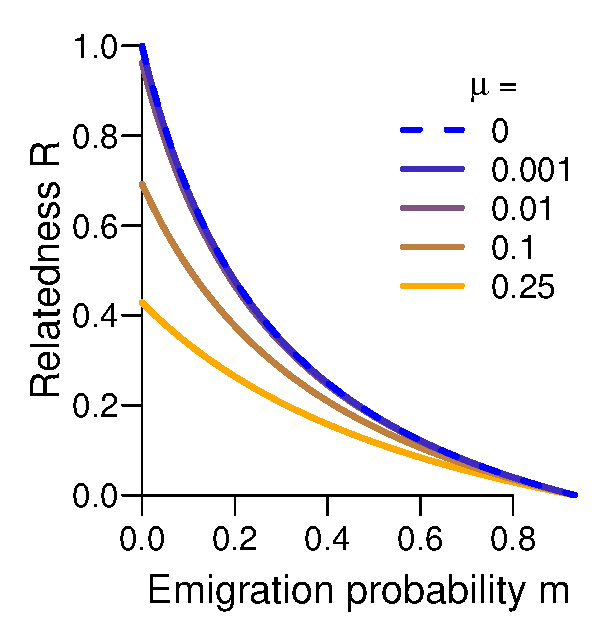
\includegraphics[width = \wpic]{../Programs/R/Pics/RplotM.pdf}}
&
\subfigure[\label{fig:sub:RWF}Wight-Fisher]{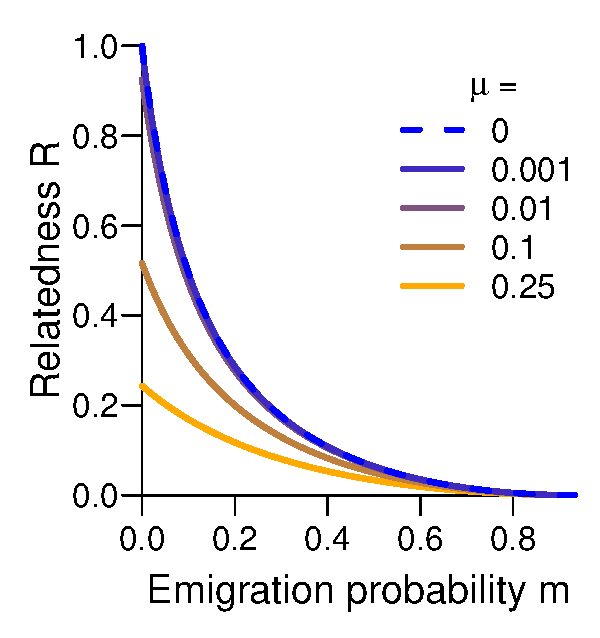
\includegraphics[width = \wpic]{../Programs/R/Pics/RplotWF.pdf}}
\end{tabular}
\caption{Within-deme relatedness of pairs of individuals $R$, as a function of the emigration probability $m$, for different values of the mutation probability $\mu$ (from $0$ [blue] to $0.25$ [orange]), and for the two types of life-cycles (\subref{fig:sub:QM}: Moran, \subref{fig:sub:QWF}: Wright-Fisher). Other parameters: $n=4$ individuals per deme, $\ndemes = 15$ demes.}
\label{fig:R}
\end{figure}
   
 
%All of these terms depend on the chosen life-cycle, and on parameters such as the mutation probability $\mu$ and the emigration probability $m$. 

\subsection*{Primary and secondary effects}


We now turn to the $\mathcal{B}$ and $-\mathcal{C}$ terms of \eqref{eq:EXapprox}, which also depend on the chosen life-cycle. We further decompose these terms into primary (subscript $\prim$) and secondary (subscript $\secd$) effects \citep{WestGardner2010}: 
\begin{equation}
\begin{array}{rccc}
\mathcal{B} =&  \mathcal{B}_{\prim} &+& \mathcal{B}_{\secd},\\
-\mathcal{C} =& \underbrace{-\mathcal{C}_{\prim}}_{\textrm{Primary effect}} &+& \underbrace{-\mathcal{C}_{\secd}.}_{\textrm{Secondary effect}}
%
\end{array}
\end{equation} 
%
Primary effects correspond to unmediated consequences of interactions (they are included in $\derivn{W}{f_{\focal}}$). Secondary effects correspond to consequences of interactions mediated by other individuals, including competition. 


\subsubsection*{Primary effects}
%
Primary effects are the same for all the life-cycles that we consider:
\begin{subequations}
\begin{align}
\mathcal{B}_{\prim}^{\BD} = \mathcal{B}_{\prim}^{\DB} = \mathcal{B}_{\prim}^{\WF} &= (1-\mu) \bb, \\
-\mathcal{C}_{\prim}^{\BD} = -\mathcal{C}_{\prim}^{\DB} = -\mathcal{C}_{\prim}^{\WF} &= (1-\mu) (-\cc),
\end{align}
\end{subequations}
%
and they do not depend on the emigration probability $m$ (see \appname~\ref{sec:app:dW} for details of the calculations). 

As we have seen above, the relatedness terms $R^{\Moran}$ and $R^{\WF}$ decrease with $m$ (keeping $m<1 - 1/\ndemes$; see figure~\ref{fig:R}). Consequently, if we ignored secondary effects, we would conclude that the expected frequency of altruists in the population $\Esp{\overline{X}}$ decreases as the emigration probability $m$ increases. However, secondary effects play a role as well.

\subsubsection*{Secondary effects}

Secondary effects take competition into account, that is, how the change in the fecundity of an individual affects the fitness of another one. As shown already in models with nearly perfect strategy transmission \citep{GrafenArchetti2008}, competition terms depend on the chosen life-cycle, because life-cycle details affect the distance at which competitive effects are felt. Given the way the model is formulated, $-\mathcal{C}_{\secd} = \mathcal{B}_{\secd}/(n-1)$ holds for all the life-cycles that we consider (see \appname~\ref{sec:app:dW} for details of the calculations). 

Under the Moran Birth-Death life-cycle, both the probability of reproducing and the probability of dying depend on the composition of the population. We obtain the following secondary effects: 
\begin{subequations}\label{eq:secondary}
\begin{equation}\label{eq:BDsec}
-\mathcal{C}_{\secd}^{\BD} = \frac{\mathcal{B}_{\secd}^{\BD}}{n-1}= - (\bb - \cc) \left( -\dfrac{\mu}{N} + \dfrac{1-m}{n} \right).
\end{equation}

The competitive effects are the same for the Moran Death-Birth and Wright-Fisher life-cycles. In both cases, the probabilities of dying are constant, so we can factor $(1-\mu)$ in the equations:
\begin{equation}\label{eq:DBsec}
-\mathcal{C}_{\secd}^{\DB} = \frac{\mathcal{B}_{\secd}^{\DB}}{n-1}= -\mathcal{C}_{\secd}^{\WF} = \frac{\mathcal{B}_{\secd}^{\WF}}{n-1}=
- (\bb - \cc) (1-\mu) \left( \frac{(1-m)^2}{n} + \frac{m^2}{N-n}\right). 
\end{equation}
\end{subequations}

These secondary effects (\eqref{eq:BDsec} and \eqref{eq:DBsec}) remain negative for the range of emigration values that we consider ($0<m<1-1/\ndemes)$, and increase with $m$. In other words, the intensity of competition decreases as emigration $m$ increases.

While the value of these secondary effects increases with emigration $m$, relatedness $R$, by which they are eventually multiplied in \eqref{eq:EXapprox}, decreases with $m$. We therefore cannot determine the overall effect of emigration $m$ on the expected frequency of altruists in the population by inspecting the different terms of \eqref{eq:EXapprox} in isolation. For each life-cycle, we need to consider the entire equations to know the overall effect of the emigration probability $m$ on the expected frequency of altruists $\Esp{\overline{X}}$ and on how it is affected by the (in)fideliy of parent-offspring transmission $\mu$. 
 
\subsection*{Changes of the expected frequency of altruists with the emigration probability $m$} 

The rather lengthy formulas that we obtain are relegated to the \appname{} and supplementary Mathematica file, and we concentrate here on the results. 

\subsubsection*{Moran Birth-Death}

For the Moran Birth-Death life-cycle, we find that the expected frequency of altruists $\Esp{\overline{X}}$ is a monotonic function of the emigration probability $m$. The direction of the change depends on the value of the mutation probability $\mu$ compared to a threshold value $\mu_c^{\BD}$. When $\mu<\mu_c^{\BD}$, $\Esp{\overline{X}}$ decreases with $m$, while when $\mu>\mu_c^{\BD}$, $\Esp{\overline{X}}$  increases with $m$. The critical value $\mu_c^{\BD}$ is given by 
\begin{equation}\label{eq:mucBD}
\mu_c^{\BD} = %
1 - \frac{\bb  - \cc + \sqrt{(\bb - \cc) \left(4 \bb N^2 + \bb - \cc \right)} }{2 \bb N}
\end{equation}
%
(recall that $N$ is the total size of the population, $N=n \ndemes$.) This result is illustrated in figure~\ref{fig:EX}\subref{fig:EXBD}; with the parameters of the figure, $\mu_c^{\BD} \approx 0.026$. The threshold value increases with both deme size $n$ and number of demes $\ndemes$, up to a maximum value $1 - \sqrt{1-\cc/\bb}$ (equal to $0.034$ with our parameters.)

With this life-cycle however, the expected frequency of altruists $\Esp{\overline{X}}$ remains lower than $\mutbias$, its value in the absence of selection (\ie, when $\selstr =0$). 

\subsubsection*{Moran Death-Birth}

The relationship between $\Esp{\overline{X}}$ and $m$ is a bit more complicated for the Moran Death-Birth life-cycle. For simplicity, we concentrate on what happens starting from low emigration probabilities (\ie, on the sign of the slope of $\Esp{\overline{X}}$ as a function of $m$ when $m\to 0$). If the benefits $\bb$ provided by altruists are relatively low ($\bb < \cc (n+1)$), $\Esp{\overline{X}}$ initially increases with $m$ provided the mutation probability $\mu$ is greater than a threshold value $\mu_c^{\DB}$ given in \eqref{eq:mucDB} below; otherwise, when the benefits are high enough, $\Esp{\overline{X}}$ initially increases with $m$ for any value of $\mu$. Combining these results, we write
\begin{equation}\label{eq:mucDB}
\mu_c^{\DB} = \begin{cases}
\dfrac{ (n+1) \cc - \bb}{ (2 n - 1) \bb - (n-1) \cc} & \textrm{if $\bb < \cc (n+1)$,} \\
%
0 & \textrm{otherwise. }
\end{cases}
\end{equation} 
%
When $\bb < \cc (n+1)$, the mutation threshold does not depend on the number of demes $\ndemes$, but increases with deme size $n$. In figure~\ref{fig:EX}\subref{fig:EXDB}, the parameters are such that $\mu_c^{\DB} = 0$. 

When $\mu > \mu_c^{\DB}$, the expected frequency of altruists $\Esp{\overline{X}}$ reaches a maximum at an emigration probability $m_c^{\DB}$ (whose complicated equation is given in the supplementary Mathematica file), as can be seen in figure~\ref{fig:EX}\subref{fig:EXDB}. When the mutation probability gets close to $0$ ($\mu \to 0$), $m_c^{\DB}$ also gets close to $0$.

With the Death-Birth life-cycle, the expected frequency of altruists is higher than its neutral value $\mutbias$ for intermediate values of the emigration probability $m$ (unless $\mu \to 0$, in which case the lower bound tends to $0$).

\subsubsection*{Wright-Fisher}

Under a Wright-Fisher updating, the expected frequency of altruists in the population reaches an extremum at the highest admissible emigration value $m = 1-\frac{1}{\ndemes}$. This extremum is a maximum when the mutation probability is higher than a threshold value $\mu_c^{\WF}$ given by 
\begin{equation}
\mu_c^{\WF} = 1-\sqrt{1-\frac{\cc}{\bb}},
\end{equation}
and it is a minimum otherwise. With the parameters of figure~\ref{fig:EX}\subref{fig:EXWF}, $\mu_c^{\WF} = 0.034$. 

With the Wright-Fisher life-cycle however, the expected frequency of altruists remains below its value in the absence of selection, $\mutbias$. 


% Figure weak selection
\begin{figure}
\hspace{-2cm}\begin{tabular}{ccc}
\subfigure[Death-Birth \label{fig:EXDB}]{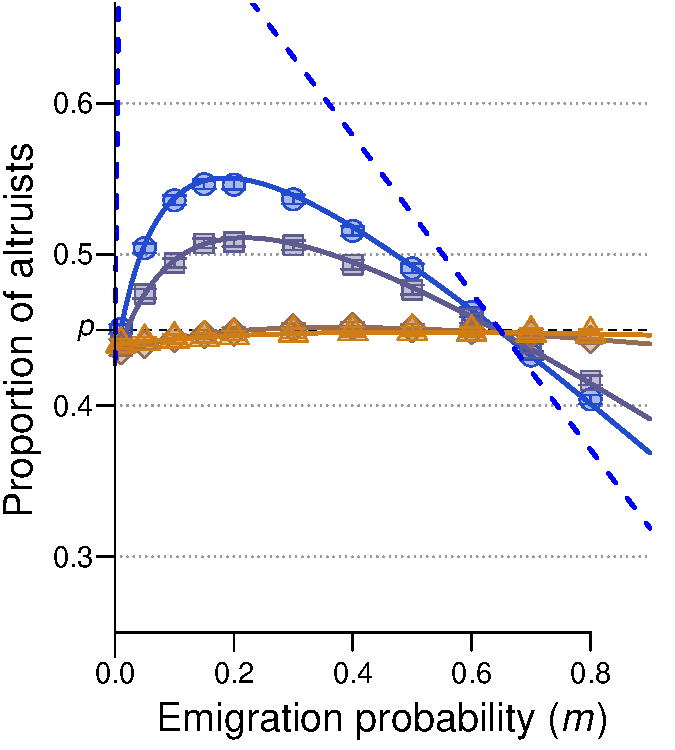
\includegraphics[type=pdf,ext=.pdf,read=.pdf, width=\wpic]{../Programs/R/Pics/EXDB_sel0.005_htg0}}
&
\subfigure[Birth-Death \label{fig:EXBD}]{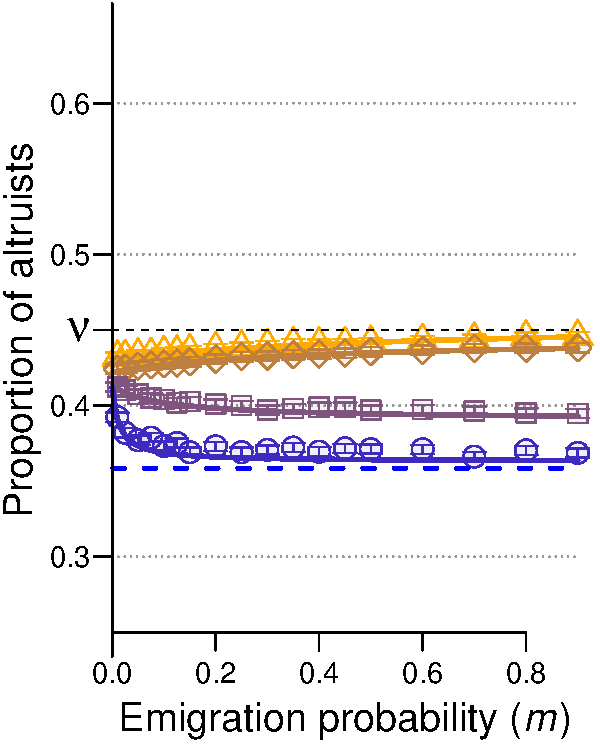
\includegraphics[type=pdf,ext=.pdf,read=.pdf, width=\wpic]{../Programs/R/Pics/EXBD_sel0.005_htg0}}
&
\subfigure[Wright-Fisher \label{fig:EXWF}]{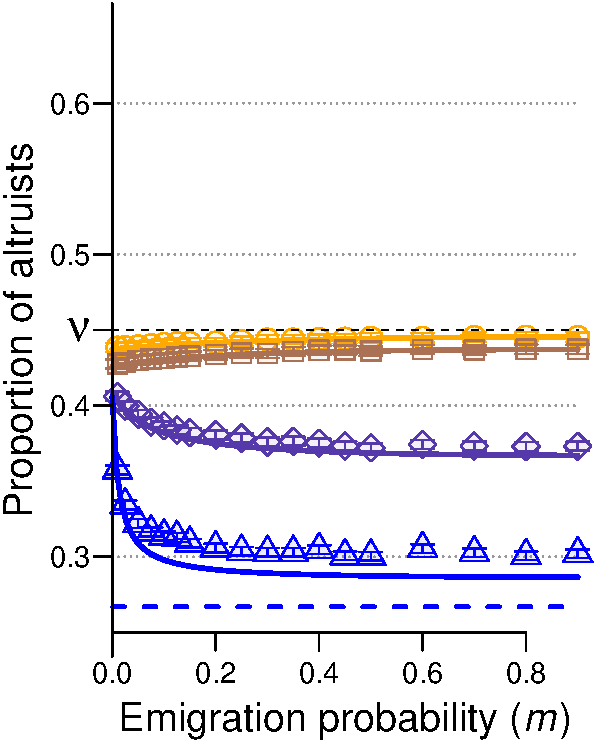
\includegraphics[type=pdf,ext=.pdf,read=.pdf, width=\wpic]{../Programs/R/Pics/EXWF_sel0.005_htg0}}
\end{tabular}
\caption{Expected proportion of altruists under weak selection, as a function of the emigration probability $m$, for different mutation values ($\mu = 0.001$ (blue, dots), $0.01$ (purple, squares), $0.1$ (brown, diamonds), $0.25$ (orange, triangles); the dashed blue lines correspond to $\mu=0$) and different life-cycles (\subref{fig:EXDB} Moran Death-Birth, \subref{fig:EXBD} Moran Birth Death, \subref{fig:EXWF} Wright-Fisher). The curves are the analytical results, the points are the output of numerical simulations. 
Parameters: $\selstr = 0.005$, $\mutbias=0.45$, $b = 15$, $c = 1$, $n=4$ individuals per deme, $\ndemes=15$ demes.}
\label{fig:EX}
\end{figure}


\subsection*{Relaxing key assumptions}

To derive our analytical results, we had to make a number of simplifying assumptions, such as the fact that selection is weak ($\selstr \ll 1$), and the fact that the structure of the population is regular (all demes have the same size $n$). We checked with numerical simulations the robustness of our results when these key assumptions are relaxed. 

\paragraph{Strong selection}When selection is strong, the patterns that we identified not only still hold but are even more marked, as shown on figure~\ref{fig:EXstrongsel}. 

\paragraph{Heterogeneity in deme sizes}To relax the assumption of equal deme sizes, we randomly drew deme sizes at the beginning of simulations, with sizes ranging from $2$ to $6$ individuals and on average $\overline{n} = 4$ individuals per deme as previously. As shown in figure~\ref{fig:EXhtg}, the patterns initially obtained with a homogeneous population structure are robust when the structure is heterogeneous. 
 
\paragraph{No self-replacement}For the Moran model, it may seem odd that an offspring can replace its own parent (which can occur since $d_{ii} \neq 0$). Figure~\ref{fig:EXdself}, plotted with dispersal probabilities preventing immediate replacement of one's own parent (for all sites $i$, $d_{ii}=\dself=0$; $\din = (1-m)/(n-1)$ for two different sites in the same deme, $\dout$ remaining unchanged), confirms that this does affect our conclusions. 

\paragraph{Infinite number of demes}Our results are obtained in a population of finite size (the figures are drawn with $\ndemes =15$ demes), but still hold when the size of the population is larger. Figure~\ref{fig:DB}\subref{fig:sub:qualit} shows the range of emigration and mutation values such that altruism is favored, plotted also for $\ndemes\to \infty$.

\paragraph{Same graphs for dispersal and social interactions} Compared to graphs classically used in evolutionary graph theory (\eg, regular random graphs, grids), the island model is particular because the interaction graph and the dispersal graph are different: interactions take place only within demes ($\eout = 0$), while offspring can disperse out of their natal deme ($\dout >0$). One may wonder whether our result depends on this difference between the two graphs. Figure~\ref{fig:EXsameDE} shows that the result still holds when the dispersal and interaction graphs are the same. In this figure indeed, we let a proportion $m$ (equal to the dispersal probability) of interactions occur outside of the deme where the individuals live, and set $\dself$, the probability of self replacement, equal to $0$, so that the dispersal and interactions graphs are the same. Our conclusions remain unchanged.



\section*{Discussion}
% Summary
\subsection*{The expected frequency of altruists in a subdivided population can increase with the probability of emigration}
Assuming that the transmission of a social strategy (being an altruist or a defector) from a parent to its offspring could be imperfect, we found that the expected frequency of altruists maintained in a population could increase with the probability $m$ of emigration out of the parental deme, a parameter tuning population viscosity. This result can seem surprising, because it contradicts the conclusions obtained under the assumption of nearly perfect strategy transmission (\ie, in the case of genetic transmission, when mutation is very weak or absent). Under nearly perfect strategy transmission indeed, increased population viscosity (\ie, decreased emigration probability) is either neutral \citep[][and dashed lines in figures~\ref{fig:EX}\subref{fig:EXBD}--\subref{fig:EXWF}]{Taylor1992islandmodel} or favorable \citep[][and dashed lines in figure~\ref{fig:EX}\subref{fig:EXDB}]{TaylorDayWild2007} to the evolution of altruistic behavior. 

\subsection*{Quantitative vs. qualitative measures}
% Measure of altruism: quanti vs quali
Often, evolutionary success is measured qualitatively, by comparing a quantity (an expected frequency, or, in models with no mutation, a probability of fixation) to the value it would have in the absence of selection. In our model, this amounts to saying that altruism is favored whenever $\Esp{\overline{X}} > \mutbias$ ($\mutbias$ is plotted as a horizontal dashed line in figure~\ref{fig:EX}). 
Some of our conclusions change if we use this qualitative measure of evolutionary success: Under the Moran Birth-Death and Wright-Fisher life-cycles, population viscosity does not promote the evolution of altruism -- actually, these two life-cycles cannot ever promote altruistic behavior for any regular population structure \citep{Taylor2011}, whichever the probability of mutation \citep{Debarre2017}. 
However, under a Moran Death-Birth life-cycle (figure~\ref{fig:EX}\subref{fig:EXDB}), altruism can be favored only at intermediate emigration probabilities. Starting for initially low values of $m$, increasing the emigration probability can still favor the evolution of altruism under this qualitative criterion (see figure~\ref{fig:DB}\subref{fig:sub:qualit}.)  


\subsection*{Interpreting the effect of $m$ on $\Esp{\overline{X}}$}

%When strategy transmission is perfect ($\mu\to 0$, the classically studied case), emigration has either no effect of the expected frequency of altruists in the population (under Wright-Fisher and Moran Birth-Death life-cycles, dashed lines in figure~\ref{fig:EX}\subref{fig:EXBD}, \subref{fig:EXWF}), or has a negative effect (under Moran Death-Birth, dashed line in figure~\ref{fig:EX}\subref{fig:EXDB}). 
%Here, we find thresholds of transmission (in)fidelity $\mu$ such that higher emigration probabilities can favor altruistic behavior. The result may appear counterintuitive because explanations for the effect of population viscosity on the evolution of altruism often focus on primary effects. The role played by secondary effects is harder to grasp. 
To better understand the role played by the mutation intensity $\mu$, we focus on the qualitative condition for the evolution of altruism ($\Esp{\overline{X}} > \mutbias$); and on the Death-Birth life-cycle, since this qualitative condition is not satisfied in the two other life-cycles. %
Having made sure that $\mathcal{B}^{\DB}>0$ (as shown in the supplementary Mathematical file), the qualitative condition for altruism to be favored is given by 
\begin{equation}\label{eq:BCcond}
\Esp{\overline{X}} > \mutbias \Leftrightarrow R^{\Moran} > \frac{\mathcal{C}^{\DB}}{\mathcal{B^{\DB}}}.
\end{equation}
%
With the Death-Birth life-cycle, the $\mathcal{C}^{\DB}/\mathcal{B}^{\DB}$ ratio does not change with the mutation probability $\mu$ (the $(1-\mu)$ factors simplified out), but the ratio decreases with the emigration probability $m$ (with $0<m<1-1/\ndemes$; see the thick black curve in figure~\ref{fig:DB}\subref{fig:sub:explain}). This decrease of the $\mathcal{C}^{\DB}/\mathcal{B}^{\DB}$ ratio is due to secondary effects (competition) diminishing as emigration increases. Relatedness, on the other hand, decreases with both $\mu$ and $m$ (see figure~\ref{fig:DB}\subref{fig:sub:explain}). We need to explain the effect of the emigration probability $m$ on condition~\eqrefnoeq{eq:BCcond} for different values of mutation intensity $\mu$. 

When the emigration probability $m$ is high, relatedness gets closer to zero for all values of mutation intensity $\mu$, while the $\mathcal{C}^{\DB}/\mathcal{B}^{\DB}$ remains positive; condition~\eqrefnoeq{eq:BCcond} is not satisfied. On the other hand, when the emigration probability $m$ is vanishingly small, $\lim_{m\to 0} R^{\Moran} \leq \lim_{m\to 0} \frac{\mathcal{C}^{\DB}}{\mathcal{B^{\DB}}}$, the two only being equal when $\mu=0$. Hence, condition~\eqrefnoeq{eq:BCcond} is satisfied for vanishingly low $m$ only when strategy transmission is perfect. Finally, as $m$ increases to intermediate values, the $\frac{\mathcal{C}^{\DB}}{\mathcal{B^{\DB}}}$ ratio decreases with a steeper slope than relatedness $R$, so that the curves can cross provided the mutation probability $\mu$ is not too high, \ie, that $R$ was not initially too low already. Hence, for no too high mutation intensity,  there is a range of emigration values $m$ such that condition~\eqrefnoeq{eq:BCcond} is satisfied.


\begin{figure}
\begin{tabular}{cc}
\subfigure[\label{fig:sub:explain}]{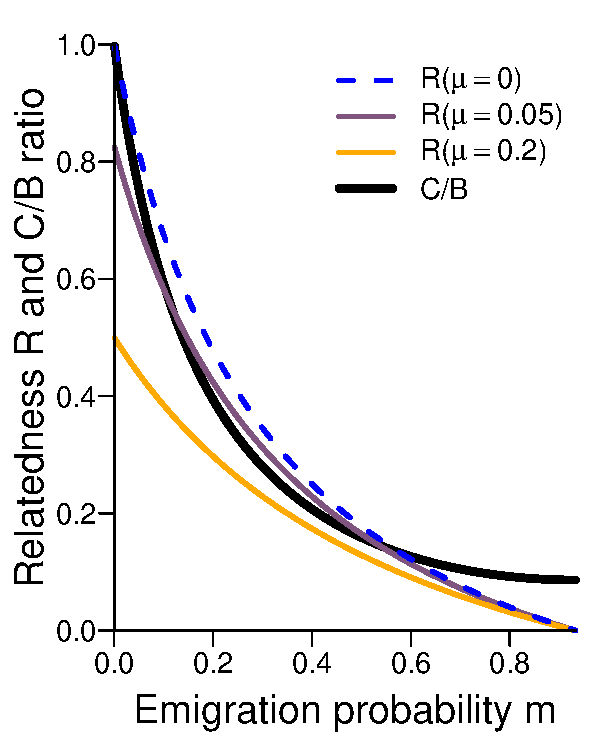
\includegraphics[width = \wpic]{../Programs/R/Pics/explainDB.pdf}}
&
\subfigure[\label{fig:sub:qualit}]{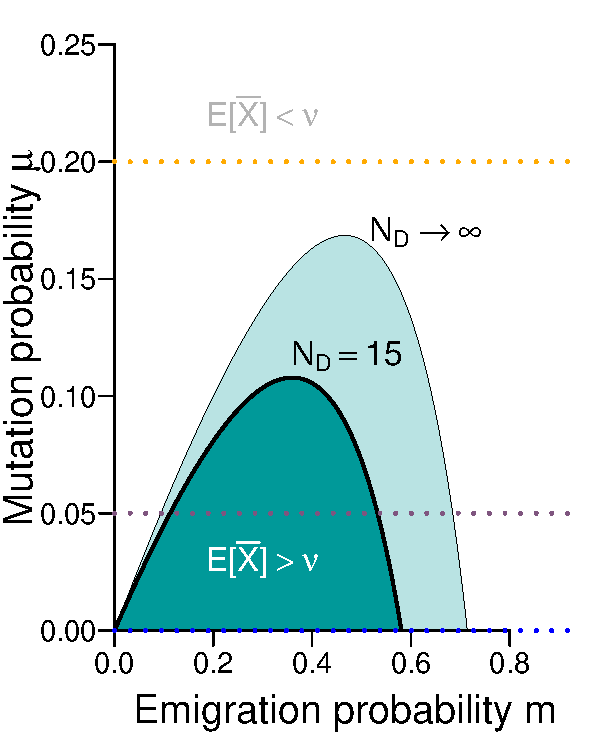
\includegraphics[width = \wpic]{../Programs/R/Pics/qualitDB.pdf}}
\end{tabular}
\caption{Understanding the effect of emigration $m$ on whether altruism is favored in the Death-Birth life-cycle. \subref{fig:sub:explain} Comparison of the $\mathcal{C}/\mathcal{B}$ ratio (thick black curve) and relatedness $R$ (thin curves) for different values of the mutation probability $\mu$ (same color code as previously). \subref{fig:sub:qualit} ($m$, $\mu$) combinations for which $\Esp{\overline{X}}>\mutbias$. The dotted horizontal lines correspond to the mutation values used in panel \subref{fig:sub:explain}. Unless specified, all other parameters are the same as in figure~\ref{fig:EX}.
}
\label{fig:DB}
\end{figure}


% How to explain the result
\subsection*{The result is due to secondary effects}
The result, that frequency of altruists can increase with the emigration probability $m$, may seem counterintuitive. It is the case because verbal explanations for the evolution of altruism often rely on primary effects only. Relatedness $R$ decreases with $m$, so it may be tempting to conclude that increases in the emigration probability $m$ are necessarily detrimental to the evolution of altruism. However, secondary effects play an opposite role, as competition decreases with $m$, and the effect is strongest at low values of $m$ (see the black curve on figure~\ref{fig:DB}\subref{fig:sub:explain}; in the absence of secondary effects, it would just be a horizontal line). %To further explain the relative weight of the detrimental and beneficial consequences of increases in the emigration probability $m$, let us focus on the Death-Birth life-cycle and consider the qualitative criterion for evolutionary success ($\Esp{\overline{X}}>\mutbias$, \ie{} $R > \mathcal{C}/\mathcal{B}$; figure~\ref{fig:DB}.)

%When parent-offspring strategy transmission is nearly perfect ($\mu \to 0$), for vanishingly small emigration probabilities ($m \to 0$), both $R$ and the $\mathcal{C}/\mathcal{B}$ ratio tend to $1$. An increase in the mutation probability $\mu$ reduces $R$ while leaving $\mathcal{C}/\mathcal{B}$ unchanged. In other words, for vanishingly small emigration probabilities, altruism is favored by selection only when transmission fidelity is nearly perfect. Let us now consider that benefits $\bb$ of social interactions are high enough for altruism to be favored at low $m$ when $\mu \to 0$ (as in figure~\ref{fig:DB}\subref{fig:sub:explain}). Starting from low values of $m$, small increases in $m$ have a stronger effect on the $\mathcal{C}/\mathcal{B}$ ratio than on relatedness $R$: local competition is initially so strong that the beneficial reduction in competition caused by an increase in $m$ initially predominates over the detrimental reduction in relatedness $R$. The opposite holds for much higher values of $m$: competition is already small enough that reducing it further does not outweigh the reduction in relatedness $R$. 

Secondary effects are less straightforward to understand than primary effects, and yet they play a crucial role for social evolution in spatially structured populations. Competition among relatives is for instance the reason for \citet{Taylor1992}'s cancellation result. Similarly, the qualitative differences between the Moran Birth-Death and Moran Death-Birth life-cycles is explained by the different scales of competition that the two life-cycle produce \citep{GrafenArchetti2008, DebarreHD2014}. Secondary effects are also behind the evolution of social behaviors such as spite \citep{WestGardner2010}. 

%  To simplify the explanations, let us consider that the number of demes is large: in this case, $\Qout$ is vanishingly small. Let us also assume that there is no direct cost to being an altruist ($\cc = 0$). 

\subsection*{Other model}
% Order of limits
\subsection*{How small is small and how large is large?}
Our results were derived under the assumption of weak selection, assuming that the phenotypic difference between altruists and defectors is small ($\selstr \ll 1$). We considered any fidelity of transmission (any $\mu$ between $0$ and $1$) and population size. However, most models considering subdivided populations assume nearly perfect strategy transmission ($\mu \to 0$) and infinite population sizes (number of demes $\ndemes \to \infty$). The point is technical, but it is important to know that the order in which these limits are taken matters, \ie, one needs to specify how small $\mu$ and $\selstr$ are compared to the inverse size of the population $1/N$. This remark complements findings by \citet{SampleAllen2017}, who highlighted the quantitative differences between different orders of weak selection and large population limits. 

% Steve Frank and other models
\subsection*{Imperfect transmission and Rebellious Children}
Our model bears resemblance to the Rebellious Child Model by \citet{Frank1997}, who studied the evolution of a vertically transmitted cultural trait in an asexually reproducing population. In \citeauthor{Frank1997}'s model, however, relatedness $r$ is treated as a fixed parameter \citep[legend of Figure~7]{Frank1997}. 
Our model is mechanistic; relatedness $r$ necessarily depends on the mutation probability $\mu$, because probabilities of identity by descent do. 

Mutation was also previously included in models investigating the maintenance of cooperative microorganisms in the presence of cheaters \citep{Brockhurst2007, Frank2010}. In both of these models however, only loss-of-function mutation was considered, which corresponds to setting the mutation bias at $\mutbias=0$ in our model. This means that the all-cheaters state is absorbing; no matter how favored cooperators may otherwise be, in the long run, a finite population will only consist of cheaters. 

% Cultural transmission
\subsection*{Cultural transmission}
Strategy transmission does not have to be genetic: it can be cultural. In our model, strategy transmission occurs upon reproduction, so this is a case of vertical cultural transmission. 

The model could nevertheless be interpreted as a representation of horizontal transmission, if we described reproduction as an instance of an individual convincing another one to update its strategy. The Moran Death-Birth model can be interpreted as a modified imitation scheme \citep{BoydRicherson2002, Ohtsuki2006} -- with a specific function specifying who is imitated --, with mutation \citep{Kandori1993}. First, we choose uniformly at random an individual who may change its strategy; with probability $\mu$ the individual chooses a random strategy (altruistic with probability $\mutbias$), and with probability $1-\mu$ it imitates another individual. Who is imitated depends on the distance to the focal individual (with probability $m$ it is a random individual in another deme) and on the ``fecundities'' of those individuals (as shown in table~\ref{tab:BD}). With this interpretation of the updating rule however, there is not reproduction nor death anymore. 

It remains to be investigated how imperfect strategy transmission would affect the effect of population viscosity on the evolution of altruism in a model implementing both reproduction and horizontal cultural transmission \citep[as in][]{Lehmann2008}. Such a model could then contrast the effects of impecfect genetic transmission and imperfect horizontal cultural transmission. 



\subsection*{Coevolution of dispersal and social behavior}
This work also raises the question of what would happen if dispersal (\eg, the emigration probability $m$) could evolve as well. Recent work on the topic has shown that under some conditions disruptive selection could take place, leading to a polymorphism between sessile altruists and mobile defectors \citep{Parvinen2013, MullonKL2017bioRxiv}. The assumptions of these studies however  differ from ours in important ways, in that they consider continuous traits and use an adaptive dynamics framework, where, notably, mutations are assumed to be very rare. It remains to be investigated how non-rare and potentially large mutations would affect their result. 

\section*{Acknowledgements}
[redacted]
%Thanks to Charles Mullon for detailed comments on a previous version of the manuscript, and for suggesting the $\mathcal{B} R - \mathcal{C}$ decomposition. At ESEB 2017, S\'ebastien Lion suggested using the $R$ vs. $\mathcal{C}/\mathcal{B}$ comparison to interpret the result. This work was funded by a ANR-14-ACHN-0003-01 grant. 

\singlespacing
%%% ___ BIBLIO _____
\clearpage
\bibliographystyle{bibstyle}
\bibliography{bibSCSP}
\doublespacing

%\processdelayedfloats

%\makeatletter
%\efloat@restorefloats
%\makeatother

\clearpage
\setcounter{figure}{0}
\section*{Figures}

\begin{figure}[h]
\begin{tabular}{cc}
\subfigure[\label{fig:subRM}Moran]{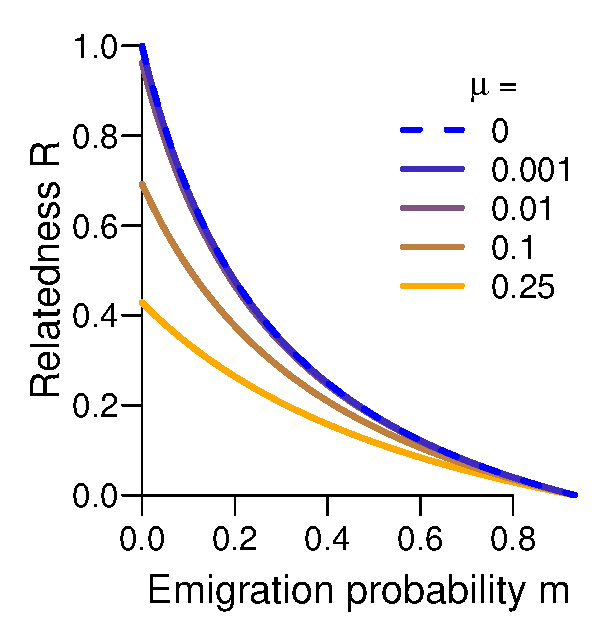
\includegraphics[width = \wpic]{../Programs/R/Pics/RplotM.pdf}}
&
\subfigure[\label{fig:sub:RWF}Wight-Fisher]{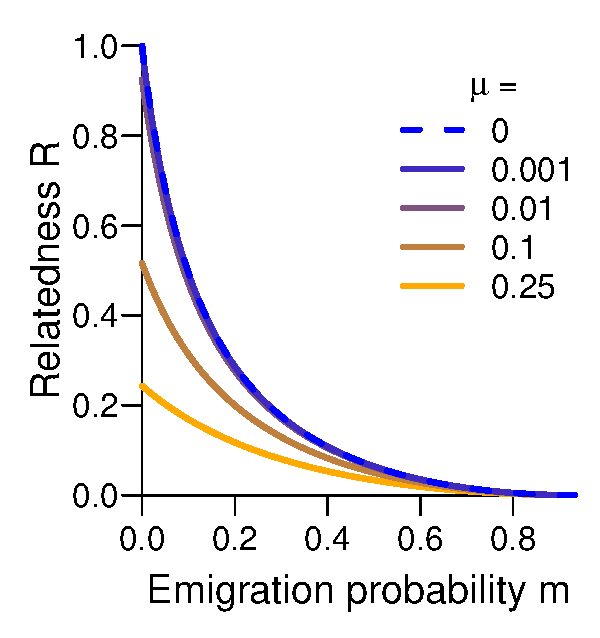
\includegraphics[width = \wpic]{../Programs/R/Pics/RplotWF.pdf}}
\end{tabular}
\caption{Within-deme relatedness of pairs of individuals $R$, as a function of the emigration probability $m$, for different values of the mutation probability $\mu$ (from $0$ [blue] to $0.25$ [orange]), and for the two types of life-cycles (\subref{fig:sub:QM}: Moran, \subref{fig:sub:QWF}: Wright-Fisher). Other parameters: $n=4$ individuals per deme, $\ndemes = 15$ demes.}
\label{fig:R}
\end{figure}

% Figure weak selection
\begin{figure}
\hspace{-2cm}\begin{tabular}{ccc}
\subfigure[Death-Birth \label{fig:EXDB}]{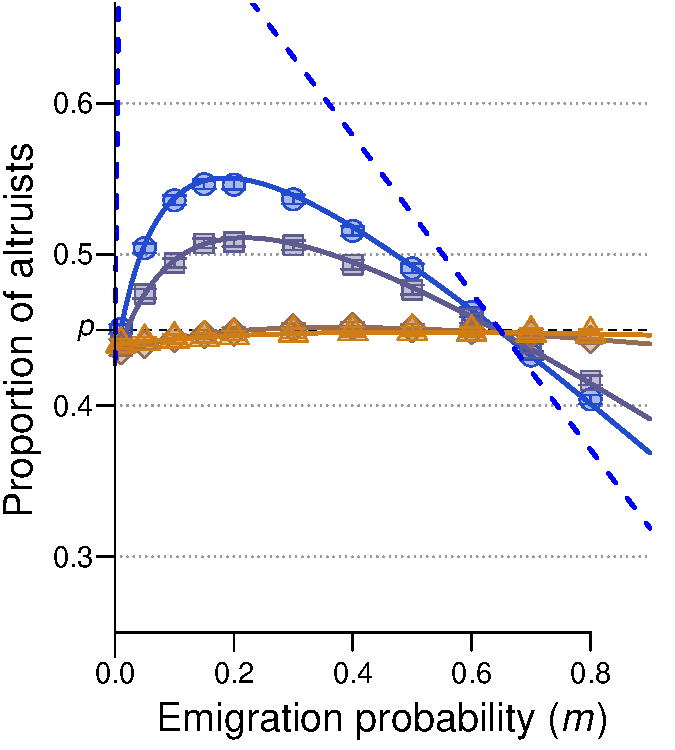
\includegraphics[type=pdf,ext=.pdf,read=.pdf, width=\wpic]{../Programs/R/Pics/EXDB_sel0.005_htg0}}
&
\subfigure[Birth-Death \label{fig:EXBD}]{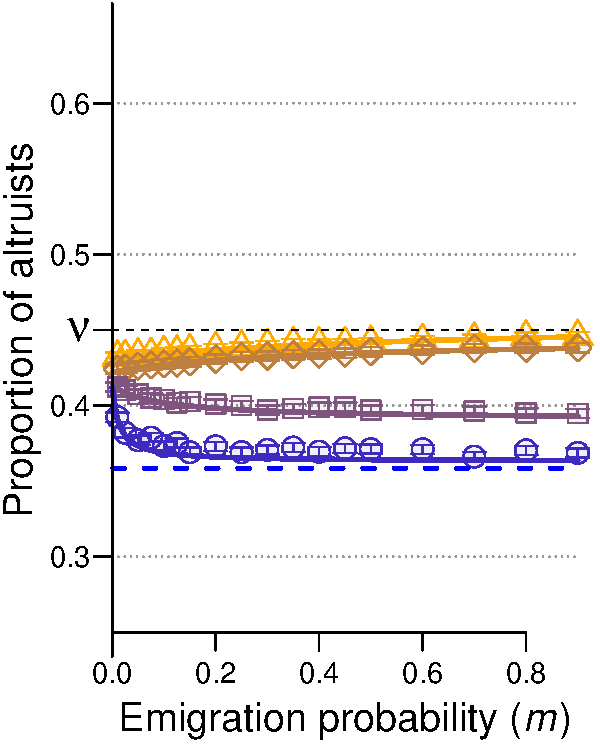
\includegraphics[type=pdf,ext=.pdf,read=.pdf, width=\wpic]{../Programs/R/Pics/EXBD_sel0.005_htg0}}
&
\subfigure[Wright-Fisher \label{fig:EXWF}]{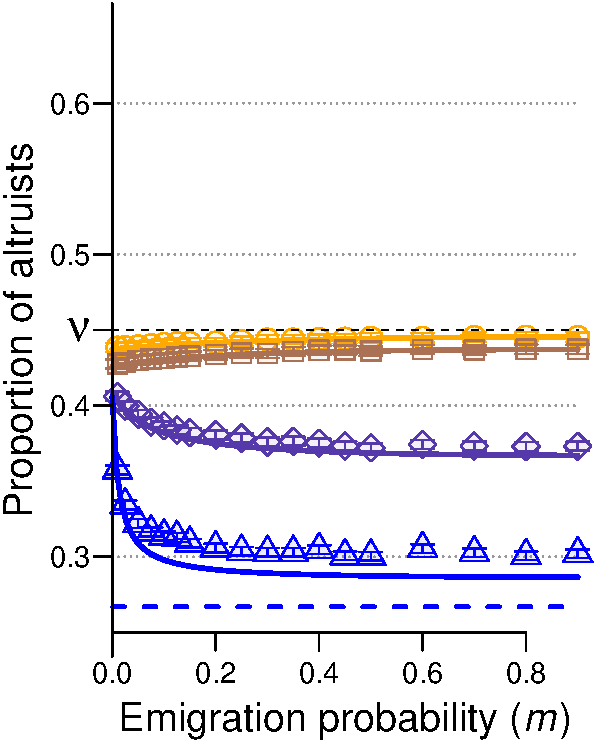
\includegraphics[type=pdf,ext=.pdf,read=.pdf, width=\wpic]{../Programs/R/Pics/EXWF_sel0.005_htg0}}
\end{tabular}
\caption{Expected proportion of altruists under weak selection, as a function of the emigration probability $m$, for different mutation values ($\mu = 0.001$ (blue, dots), $0.01$ (purple, squares), $0.1$ (brown, diamonds), $0.25$ (orange, triangles); the dashed blue lines correspond to $\mu=0$) and different life-cycles (\subref{fig:EXDB} Moran Death-Birth, \subref{fig:EXBD} Moran Birth Death, \subref{fig:EXWF} Wright-Fisher). The curves are the analytical results, the points are the output of numerical simulations. 
Parameters: $\selstr = 0.005$, $\mutbias=0.45$, $b = 15$, $c = 1$, $n=4$ individuals per deme, $\ndemes=15$ demes.}
\label{fig:EX}
\end{figure}

\begin{figure}
\begin{tabular}{cc}
\subfigure[\label{fig:sub:explain}]{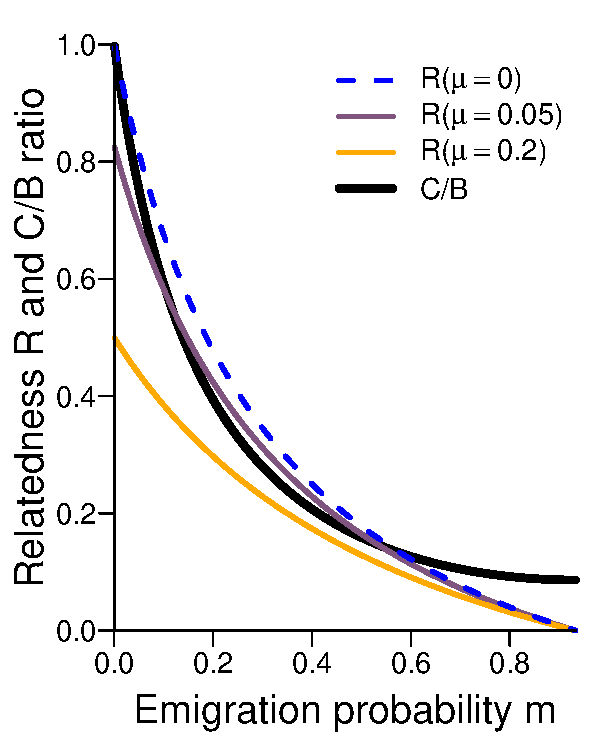
\includegraphics[width = \wpic]{../Programs/R/Pics/explainDB.pdf}}
&
\subfigure[\label{fig:sub:qualit}]{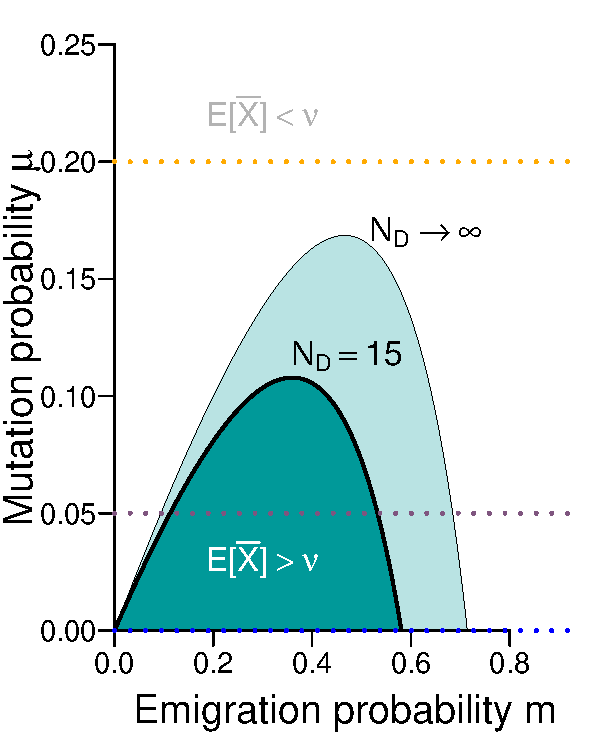
\includegraphics[width = \wpic]{../Programs/R/Pics/qualitDB.pdf}}
\end{tabular}
\caption{Understanding the effect of emigration $m$ on whether altruism is favored in the Death-Birth life-cycle. \subref{fig:sub:explain} Comparison of the $\mathcal{C}/\mathcal{B}$ ratio (thick black curve) and relatedness $R$ (thin curves) for different values of the mutation probability $\mu$ (same color code as previously). \subref{fig:sub:qualit} ($m$, $\mu$) combinations for which $\Esp{\overline{X}}>\mutbias$. The dotted horizontal lines correspond to the mutation values used in panel \subref{fig:sub:explain}. Unless specified, all other parameters are the same as in figure~\ref{fig:EX}.
}
\label{fig:DB}
\end{figure}


\clearpage
% Start the appendix

%TC:ignore 
% Ignore word count after this point

\appendix

\renewcommand{\theequation}{A\arabic{equation}}
% redefine the command that creates the equation number.
\renewcommand{\thetable}{A\arabic{table}}
\renewcommand{\thefigure}{A\arabic{figure}}
\setcounter{equation}{0}  % reset counter 
\setcounter{figure}{0}
\setcounter{table}{0}
 
\section*{Supplementary figures} 

% Figure strong selection
\begin{figure}[h!]
\begin{tabular}{ccc}
\subfigure[Death-Birth]{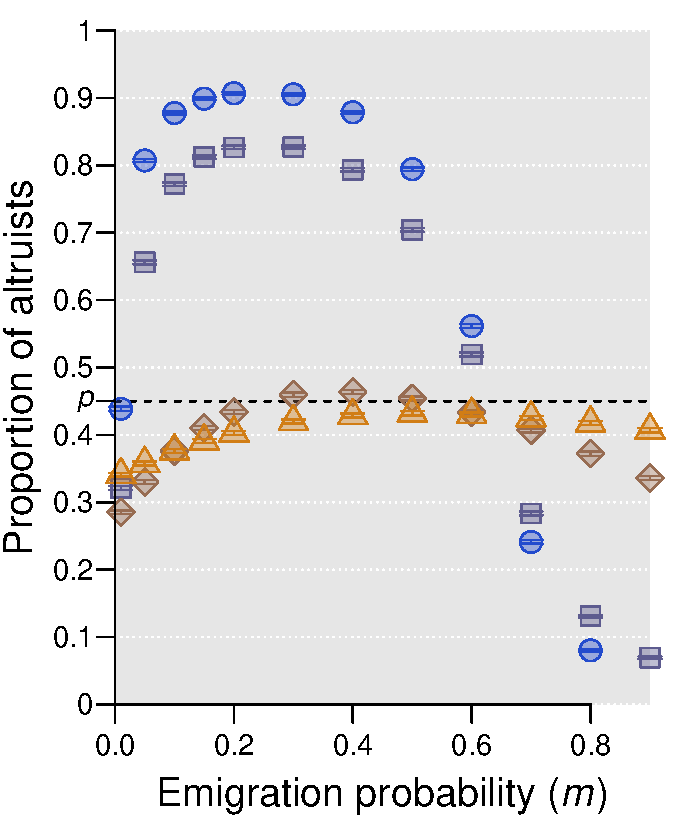
\includegraphics[type=pdf,ext=.pdf,read=.pdf, width=\wpic]{../Programs/R/Pics/EXDB_sel0.1_htg0}}
&
\subfigure[Birth-Death]{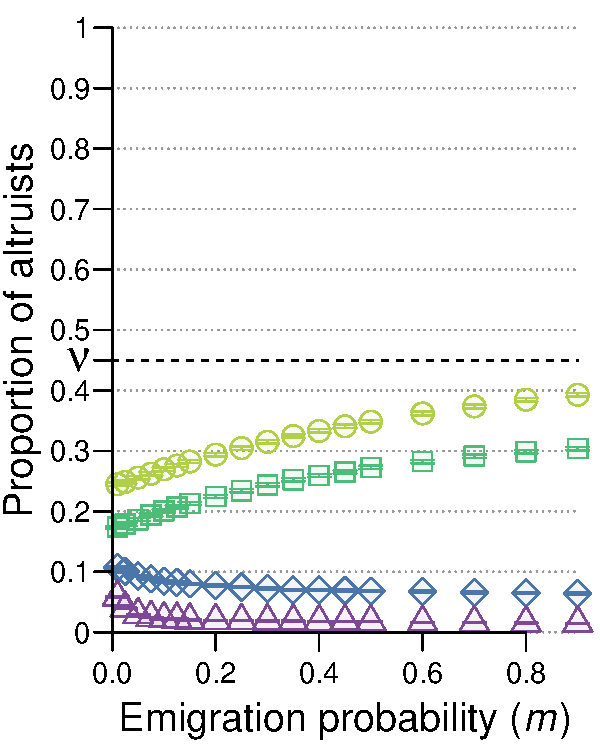
\includegraphics[type=pdf,ext=.pdf,read=.pdf, width=\wpic]{../Programs/R/Pics/EXBD_sel0.1_htg0}}
&
\subfigure[Wright-Fisher]{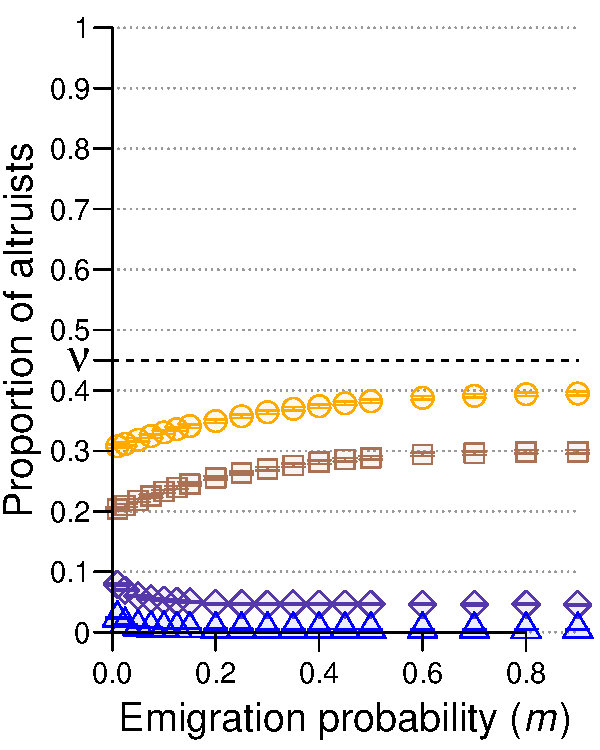
\includegraphics[type=pdf,ext=.pdf,read=.pdf, width=\wpic]{../Programs/R/Pics/EXWF_sel0.1_htg0}}
\end{tabular}
\caption{Equivalent of figure~\ref{fig:EX} (simulations only) but with strong selection ($\selstr = 0.1$); please note the change of scale on the vertical axis. All other parameters and legends are identical to those of figure~\ref{fig:EX} (increasing mutation probabilities from blue dots to orange triangles). }
\label{fig:EXstrongsel}
\end{figure}

% Figure heterogeneous population
\begin{figure}
\begin{tabular}{ccc}
\subfigure[Death-Birth]{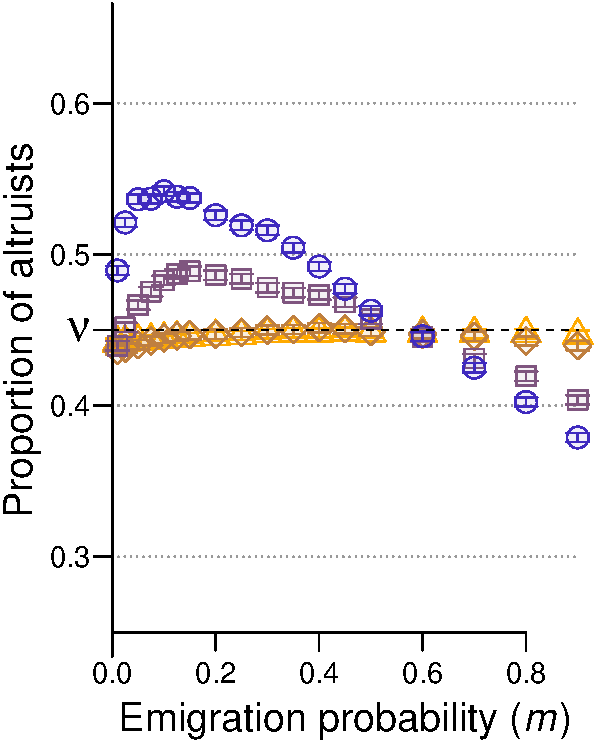
\includegraphics[type=pdf,ext=.pdf,read=.pdf, width=\wpic]{../Programs/R/Pics/EXDB_sel0.005_htg1}}
&
\subfigure[Birth-Death]{
\includegraphics[type=pdf,ext=.pdf,read=.pdf, width=\wpic]{../Programs/R/Pics/EXBD_sel0.005_htg1}}
&
\subfigure[Wright-Fisher]{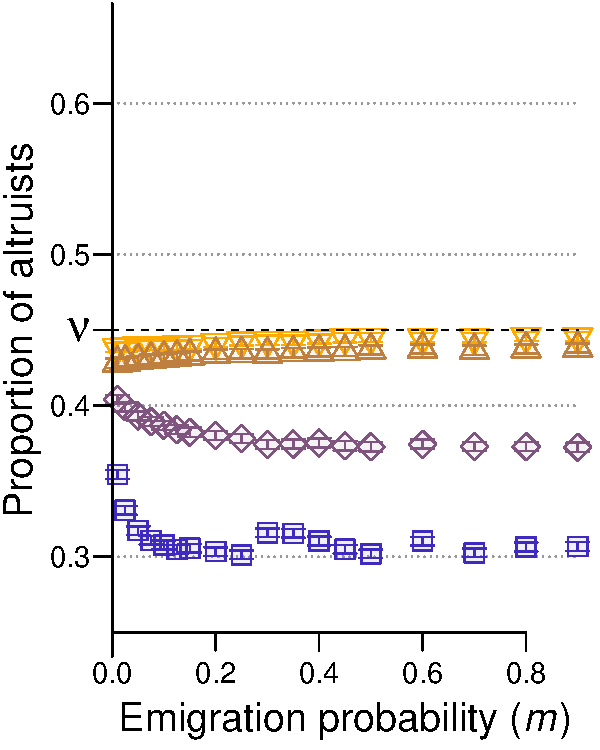
\includegraphics[type=pdf,ext=.pdf,read=.pdf, width=\wpic]{../Programs/R/Pics/EXWF_sel0.005_htg1}}\end{tabular}
\caption{Equivalent of figure~\ref{fig:EX} (simulations only) but with a heterogeneous population structure: deme sizes range from $1$ to $5$ individuals per deme, the average deme size is $4$ as in figure~\ref{fig:EX};  all other parameters and legend are identical to those of figure~\ref{fig:EX}. }
\label{fig:EXhtg}
\end{figure}


 
%\clearpage
%% Figure heterogeneous population
%\begin{figure}
%\begin{tabular}{ccc}
%\subfigure[Death-Birth]{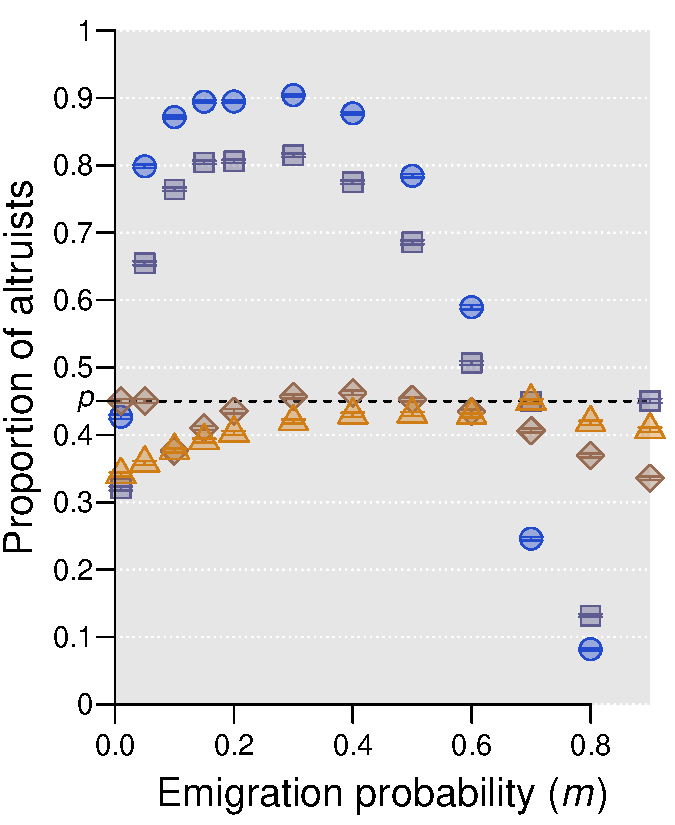
\includegraphics[type=pdf,ext=.pdf,read=.pdf, width=\wpic]{../Programs/R/Pics/EXDB_sel0.1_htg1}}
%&
%\subfigure[Birth-Death]{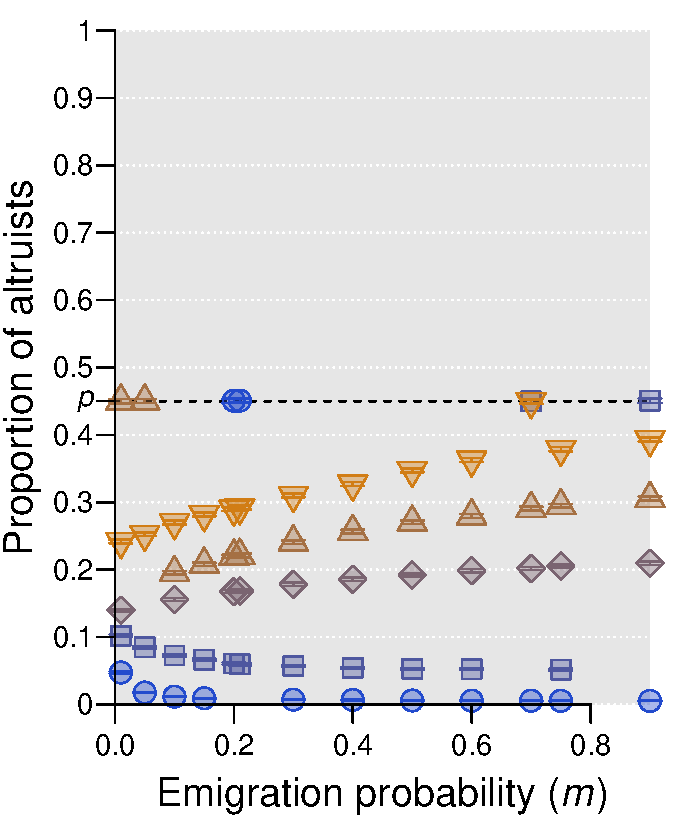
\includegraphics[type=pdf,ext=.pdf,read=.pdf, width=\wpic]{../Programs/R/Pics/EXBD_sel0.1_htg1}}
%&
%\subfigure[Wright-Fisher]{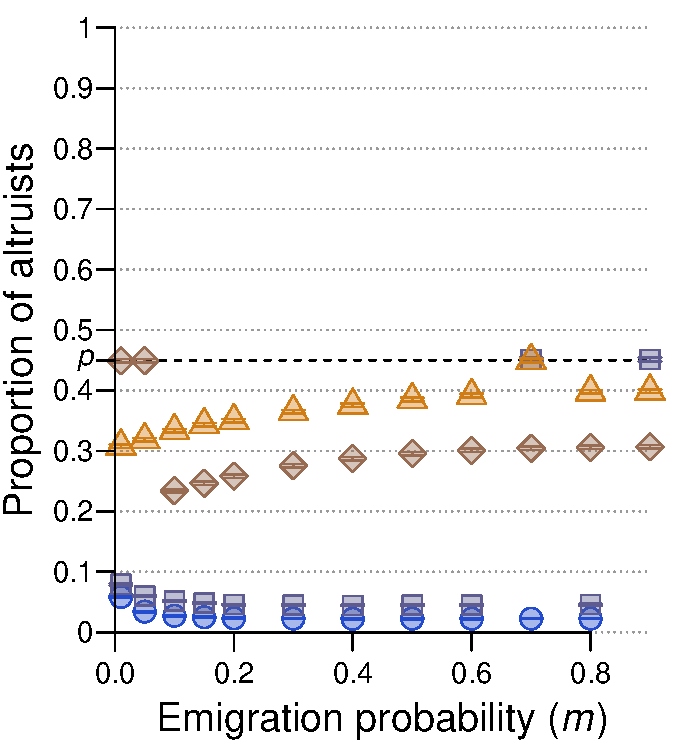
\includegraphics[type=pdf,ext=.pdf,read=.pdf, width=\wpic]{../Programs/R/Pics/EXWF_sel0.1_htg1}}\end{tabular}
%\caption{Strong selection, heterogeneous population}
%\label{fig:island_htgpop}
%\end{figure}



% Figure dself = 0
\begin{figure}
\begin{tabular}{ccc}
\subfigure[Death-Birth \label{fig:EXdselfDB}]{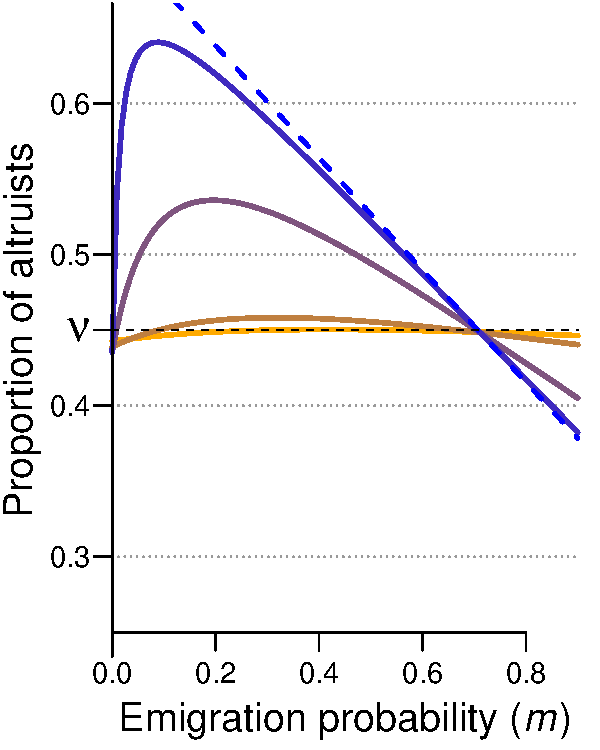
\includegraphics[type=pdf,ext=.pdf,read=.pdf, width=\wpic]{../Programs/R/Pics/EXDB_sel0.005_htg0_nodself}}
&
\subfigure[Birth-Death \label{fig:EXdselfBD}]{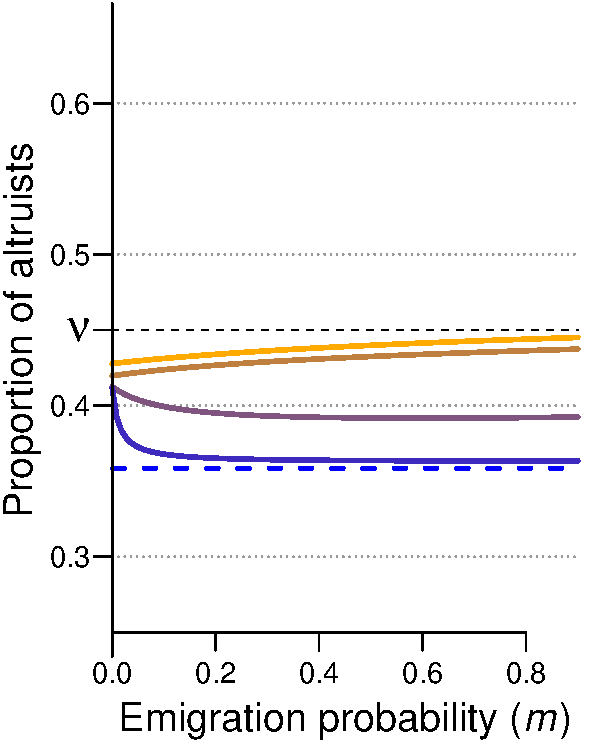
\includegraphics[type=pdf,ext=.pdf,read=.pdf, width=\wpic]{../Programs/R/Pics/EXBD_sel0.005_htg0_nodself}}
&
\subfigure[Wright-Fisher \label{fig:EXdselfWF}]{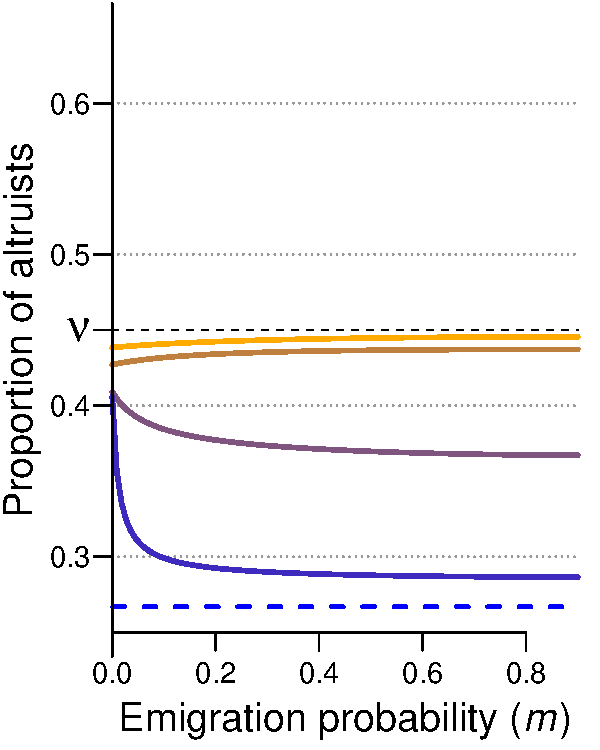
\includegraphics[type=pdf,ext=.pdf,read=.pdf, width=\wpic]{../Programs/R/Pics/EXWF_sel0.005_htg0_nodself}}
\end{tabular}
\caption{Equivalent of figure~\ref{fig:EX} (analysis only), with no self-replacement ($d_{ii} = \dself = 0$ for all sites). }
\label{fig:EXdself}
\end{figure}

% Figure SameDE
\begin{figure}
\begin{tabular}{ccc}
\subfigure[Death-Birth \label{fig:EXsameDEDB}]{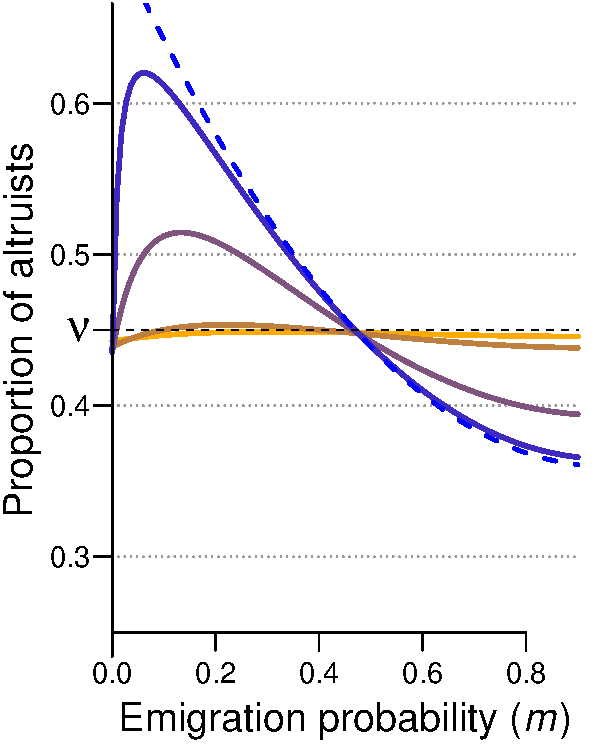
\includegraphics[type=pdf,ext=.pdf,read=.pdf, width=\wpic]{../Programs/R/Pics/EXDB_sel0.005_htg0_nodself_sameDE}}
&
\subfigure[Birth-Death \label{fig:EXsameDEBD}]{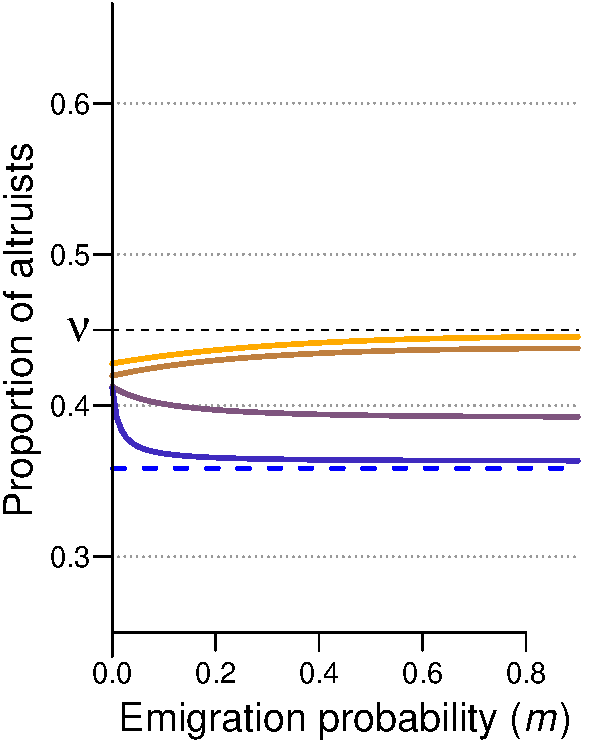
\includegraphics[type=pdf,ext=.pdf,read=.pdf, width=\wpic]{../Programs/R/Pics/EXBD_sel0.005_htg0_nodself_sameDE}}
&
\subfigure[Wright-Fisher \label{fig:EXsameDEWF}]{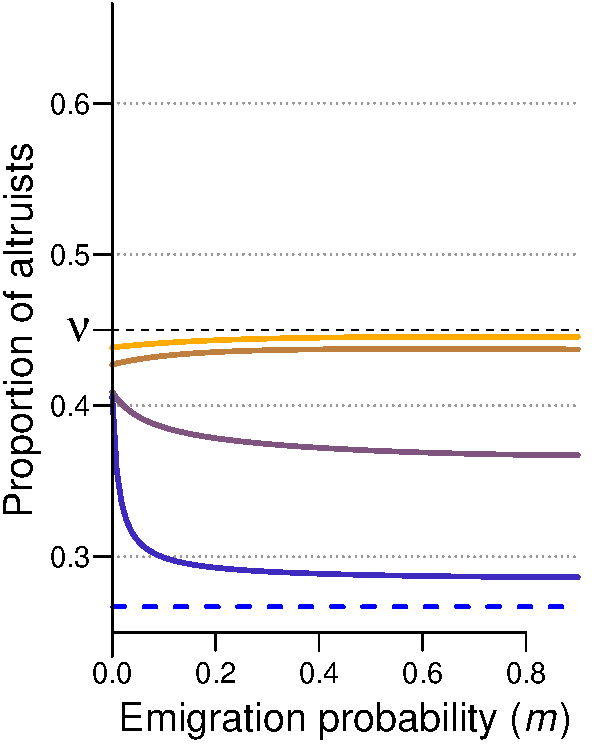
\includegraphics[type=pdf,ext=.pdf,read=.pdf, width=\wpic]{../Programs/R/Pics/EXWF_sel0.005_htg0_nodself_sameDE}}
\end{tabular}
\caption{Equivalent of figure~\ref{fig:EX} (analysis only), with equal dispersal and interaction graphs (\ie, no self-replacement [$d_{ii} = \dself = 0$ for all sites], and a proportion~$m$ of the interactions occurring outside of the home deme). }
\label{fig:EXsameDE}
\end{figure}

\clearpage
\section*{Supplementary Table}

\begin{table}[h!]
\begin{tabular}{>{$}c<{$} l}
\bb & Sum of the marginal effects of deme-mates' phenotypes on focal individual's fecundity (benefit)\\
\mathcal{B} & Sum of the marginal effects of deme-mates' phenotypes on the fitness $W$ of a focal individual\\
B_i & Expected number of successful offspring of the individual living at site $i$ (r.v.)\\
B^* & Value of $B_i$ for all sites, in the absence of selection ($\selstr = 0$)\\
\cc & Marginal effect of a focal individual's phenotype on its own fecundity (cost)\\
\mathcal{C} & Marginal effect of an individual's phenotype on its own fitness $W$\\
d_{ij} & Dispersal probability from site $i$ to site $j$\\
D_i & Probability that the individual currently living at site $i$ is dead at the end of the time step (r.v.)\\
e_{ij} & Interaction probability from site $i$ to site $j$ \\
f_i & Fecundity of the individual currently living at site $i$ (r.v.)\\
n & Deme size\\
\ndemes & Number of demes \\
N & Total population size ($N = \ndemes n$) \\
m & Emigration probability\\
P_{ij} & (Long-term) Expected state of the pair of sites ($i$,$j$)\\
Q_{ij} & (Long-term) Probability of identity by descent of individuals at sites $i$ and $j$\\
R & Pairwise within-deme relatedness (see \eqref{eq:EXapprox})\\
W_i & Measure of fitness, counting offspring only when unmutated (see \eqref{eq:defW})\\ 
X_i & Indicator variable, equal to $1$ if site $i$ is occupied by an altruist, to $0$ otherwise (r.v.)\\
\overline{X} & Frequency of altruists in the population (r.v.)\\
%\beta & Term associated to the benefits $\bb$\\
%\gamma & Term associated to the costs $\cc$ \\
\selstr & Phenotypic distance between altruists and defectors; strength of selection\\
\phi_i & Phenotype of the individual living at site $i$; $\phi_i = \selstr X_i$ (r.v.)\\
\mu & Mutation probability\\
\mutbias & Mutation bias: probability that mutant is altruist\\
\hline
\small \prim & Subscript corresponding to primary effects\\
\small \secd & Subscript corresponding to secondary effects\\
\small{\focal} & Subscript used to denote a focal individual\\
\small{\inn} & Subscript used when $i\neq j$ and the two sites are in the same deme\\
\small{\out} & Subscript used when the two sites $i$ and $j$ are in different demes\\
\small{\self} & Subscript used when $i=j$\\
\small{0} & Sub- or superscript meaning that a quantity is evaluated at $\selstr=0$ \\
\hline
\small{\BD} & Superscript corresponding to the Moran Birth-Death model\\
\small{\DB} & Superscript corresponding to the Moran Death-Birth model\\
\small{\Moran} & Superscript corresponding to a Moran model\\
\small{\WF} & Superscript corresponding to the Wright-Fisher model
\end{tabular}
\caption{List of symbols. ``r.v.'' means \textit{random variable}. }
\label{tab:symbols}
\end{table}
\clearpage

%
\singlespace

\begin{center}
{\LARGE \bfseries \appname}
\end{center}


%\newpage
\pagestyle{appendix}


\section{Mutation parameters\label{sec:app:mutation}}

In the main text, we first introduce effective mutation parameters: $\mu_{1\to 0}$, the probability that an altruist has defector offspring, and $\mu_{0\to 1}$, the probability that a defector has altruist offspring. 

\subsection{Expected frequency of altruists at the mutation-drift balance \label{sec:app:defnu}}
We assume that there is no selection acting ($\delta=0$), but that there still are two types of individuals in the population. \\
Let $Y$ be the type of a randomly chosen individual  in the population, given a proportion $y$ of altruists in the population. In expectation, we have
\begin{subequations}
\begin{equation}
\Esp{Y} = y.
\end{equation}
%
Let $Y'$ be the type of a randomly chosen individual at the next time step, given the frequency $y$ at the previous time step. This randomly chosen individual is altruist if its parent was ($y$) and it did not mutate ($\mu_{1\to 0}$), or if its parent was not altruist ($1-y$), but the offspring mutated into one ($\mu_{0\to 1}$). We obtain
%
\begin{equation}
\Esp{Y'} = y (1-\mu_{1\to 0}) + (1-y) \mu_{0\to 1}.
\end{equation}
\end{subequations}
%
The expected frequency of altruists, denoted by $\nu$, is found by solving $\Esp{Y} = \Esp{Y'}$. We obtain
%
\begin{equation}
\mutbias = \frac{\mu_{0\to 1}}{\mu_{1\to 0 }+\mu_{0\to 1}}. \label{eq:app:nuformula}
\end{equation}

\subsection{Parent-offspring correlation at the mutation drift balance}

We can then compute the parent-offspring type correlation at the mutation-drift balance. First, let us compute parent-offspring covariance:
%
\begin{equation}\label{eq:app:Cov}
\begin{aligned}
\Cov{Y Y'} &= \Esp{Y Y'} - \Esp{Y'}\Esp{Y}\\
& = \mutbias (1-\mu_{1\to 0}) - \left(\mutbias (1-\mu_{1\to 0}) + (1-\mutbias) \mu_{0\to 1}\right) \mutbias \\
%
& = \mutbias (1-\mutbias) (1 - \mu_{1\to 0} - \mu_{0\to 1}).
\end{aligned}
\end{equation}

Then, the standard deviations are given by 
\begin{equation}\label{eq:app:SD1}
\begin{aligned}
\sigma_Y &= \sqrt{\Esp{Y^2} - \Esp{Y}^2} = \sqrt{\Esp{Y} - \Esp{Y}^2} \\
& = \sqrt{\mutbias (1-\mutbias)},
\end{aligned}
\end{equation}
and
\begin{equation}\label{eq:app:SD2}
\begin{aligned}
\sigma_{Y'} &= \sqrt{\Esp{Y'^2} - \Esp{Y'}^2}  = \sqrt{\Esp{Y'} - \Esp{Y'}^2} \\
& = \sqrt{\mutbias (1-\mutbias) (1 - \mu_{1\to 0} - \mu_{0\to 1}) - (\mutbias (1-\mutbias) (1 - \mu_{1\to 0} - \mu_{0\to 1}))^2}.
\end{aligned}
\end{equation}

Finally, the parent-offspring correlation is given by 
\begin{displaymath}
\mathrm{Corr}\left[Y Y' \right] = \frac{\Cov{Y Y'}}{\sigma_Y \sigma_{Y'}};
\end{displaymath}
using the formulas \eqref{eq:app:Cov}--(\ref{eq:app:SD2}), and replacing $\mutbias$ by its value (mutation-drift equilibrium, \eqref{eq:app:nuformula}), we obtain
\begin{equation}
\mathrm{Corr}\left[ Y Y' \right] = 1 - (\mu_{1\to 0} + \mu_{0\to 1})= 1-\mu.
\end{equation}

\subsection{Redefining the mutation scheme\label{sec:app:mutnew}}

With the new mutation parameters $\mu$ and $\mutbias$, we can describe the mutation scheme differently. 

If we denote by $X_i$ the type of a given parent, then the expected type of one of its offspring is
\begin{subequations}
\begin{equation}\label{eq:app:expoff}
\Esp{X_i'|X_i} = X_i (1-\mu_{1\to 0}) + (1-X_i) \mu_{0 \to 1}. 
\end{equation}
Replacing $\mu_{1\to 0}$ and $\mu_{0\to 1}$ by equivalent combinations of $\mu$ and $\nu$, \ie, 
\begin{equation}
\mu_{1\to 0} = \mu (1-\nu) \textrm{ and } \mu_{0\to 1} = \mu \nu,
\end{equation}
then \eqref{eq:app:expoff} becomes
\begin{equation}\label{eq:app:expoff2}
\Esp{X_i'|X_i} = X_i (1-\mu) + \mu \nu. 
\end{equation}
\end{subequations}
We can redefine the mutation scheme and interpret \eqref{eq:app:expoff2} as follows. Parents transmit their strategy to their offspring with probability $1-\mu$; with probability $\mu$, offspring do not inherit their strategy from their parent but instead get one randomly: with probability $\mutbias$, they become altruists, with probability $1-\mutbias$ they become defectors. With this alternative description, we can call ``mutants'' individuals who have the same type as their parent. 

\clearpage
\section{Expected frequency of altruists\label{sec:app:EX}}

%\textit{Note: The calculation steps are the same as the ones presented in \citet{Debarre2017}; they are presented here so that the article is self-contained, but there are no new results in \appname~\ref{sec:app:EX}. }

%In this section, we work with a generic regular population structure (with symmetries such that all individuals behave the same way in expectation), of which the island model is a particular case. 

\subsection{For a generic life-cycle \label{sec:app:generic}}

We want to compute the expected proportion of altruists in the population. We represent the state of the population at a given time $t$ using indicator variables $X_i(t)$, $1\leq i \leq N$, equal to~$1$ if the individual living at site $i$ at time $t$ is an altruist, and equal to~$0$ if it is a defector; these indicator variables are gathered in a $N$-long vector $\mathbf{X}(t)$. The set of all possible population states is $\Omega = \{0,1\}^N$. The proportion of altruists in the population is written $\overline{X}(t) = \sum_{i=1}^N X_i(t)$. We denote by $B_{ji}(X(t), \selstr)$, written $B_{ji}$ for simplicity, the probability that the individual at site $j$ at time $t+1$ is the newly established offspring of the individual living at site $i$ at time $t$. The expected number of successful offspring produced by the individual living at site $i$ at time $t$ is given by $B_i = \sum_{j=1}^N B_{ji}$. We denote by $D_{i}(X(t), \selstr)$ ($D_i$ for simplicity) the probability that the individual living at site $i$ at time $t$ has been replaced (\ie, died) at time $t+1$. These quantities depend on the chosen life-cycle and on the state of the population; they are given in table~\ref{tab:BD} for each of the life-cycles that we consider. 

\begin{table}[h!]
{
\tabulinesep=1.65mm
\begin{tabu}{lcc}
\hline
Life-cycle & $B_{ji}$ & $D_i$ \\   
\hline
%
Moran Birth-Death & %
$d_{ij} \dfrac{\myphantom f_{i} \myphantom}{\sum_{k =1}^N f_{k}}$  & %
$\dfrac{\myphantom \sum_{j=1}^N d_{ji} f_j\myphantom }{\sum_{k=1}^N f_k}$ \vspace{0.em}\\
%
%
Moran Death-Birth & %
$\dfrac{1}{N}\dfrac{ d_{ij} f_i }{\sum_{k=1}^N d_{kj} f_k}$ & %
$\dfrac{1}{N}$ \vspace{0.em}
\\
%
%
Wright-Fisher & %
$\dfrac{d_{ij} f_i}{\sum_{k=1}^N d_{kj} f_k}$ & $1$
\end{tabu}
}
\caption{Formulas of $B_{ji}$ and $D_{i}$ for each of the life-cycles that we consider; $f_i$ (shorthand notation for $f_i(X, \selstr)$) is the fecundity of the individual living at site $i$, and $d_{ji}$ is a dispersal probability, given in \eqref{eq:defD}.}
\label{tab:BD}
\end{table}

Since a dead individual is immediately replaced by one new individual (\ie, population size remains constant and equal to $N$), 
\begin{subequations}
\begin{equation}\label{eq:DBequiv}
D_i = \sum_{j=1}^N B_{ij}
\end{equation}
holds for all sites $i$ and all life-cycles. 

The structure of the population is also such that in the absence of selection ($\selstr = 0$, so that $f_i=1$ for all sites $1\leq i\leq N$), all individuals have the same probability of dying and the same probability of having successful offspring (\ie, of having offspring that become adults at the next time step), so that
\begin{equation}\label{eq:DBRV}
D_i^0 = \sum_{j=1}^N B_{ji}^0= B_i^0 =: B^*, 
\end{equation}
where the $^0$ subscript means that the quantities are evaluated for $\selstr = 0$. This also implies that $B_{ij}^0$ and $D_i^0$ do not depend on the state $\mathbf{X}$ of the population. For the Moran life-cycles, $B^*=1/N$, while for the Wright-Fisher life-cycle, $B^*=1$. 
(The difference between \eqref{eq:DBRV} and  \eqref{eq:DBequiv} is that we are now considering offspring produced by $i$ landing on $j$).

\end{subequations}


Given that the population is in state $\mathbf{X}(t)$ at time $t$, the expected frequency of altruists at time $t+1$ is given by
\begin{subequations}
\begin{equation}\label{eq:conditionalchange}
\Esp{\overline{X}(t+1) | \mathbf{X}(t)} = %
\frac{1}{N} \sum_{i=1}^N \left[ B_i (1-\mu) X_i + (1-D_i) X_i + B_i \mu \mutbias  \right]. 
\end{equation}
\end{subequations}
The first term within the brackets corresponds to births of unmutated offspring from parents who are altruists ($X_i$). The second term corresponds to the survival of altruists. The third term corresponds to the births of mutants who became altruists (which occurs with probability $\mutbias$), whichever the type of the parent. 

Given that there is no absorbing population state (a lost strategy can always be recreated by mutation), there is a stationary distribution of population states; the expected frequency of altruists does not change anymore for large times~$t$ (realized frequencies of course keep changing). We denote by $\xi(\mathbf{X}, \selstr, \mu)$ the probability that the population is in state $\mathbf{X}$, given the strength of selection $\selstr$ and the mutation probability $\mu$. Taking the expectation of \eqref{eq:conditionalchange} ($\Esp{\overline{X}} = \sum_{X \in \Omega} \overline{X}\xi(\mathbf{X}, \selstr, \mu)$), we obtain, after reorganizing:
\begin{equation}\label{eq:statdist}
0 = \frac{1}{N} \sum_{X\in \Omega} \left[ \sum_{i=1}^N \left( B_i (1-\mu) X_i - D_i X_i \right) + \sum_{i=1}^N B_i \mu \mutbias \right] \xi(\mathbf{X}, \selstr, \mu). 
\end{equation}

Now, we use the assumption of weak selection ($\selstr \ll 1$) and consider the first-order expansion of \eqref{eq:statdist} for $\selstr$ close to $0$. 

\begin{equation}\label{eq:app:TaylorDetail}
\begin{aligned}
0 = & \phantom{+} \frac{1}{N} \sum_{X\in \Omega} \left[ \sum_{i=1}^N \left( B_i^0 (1-\mu) X_i - D_i^0 X_i \right) + \sum_{i=1}^N B_i^0 \mu \mutbias \right] \xi(\mathbf{X}, 0, \mu) \\
%
& + \frac{1}{N} \sum_{X\in \Omega} \left[ \sum_{i=1}^N \left( \frac{\partial B_i (1-\mu) - D_i}{\partial \selstr} X_i  \right) + \sum_{i=1}^N \frac{\partial B_i}{\partial \selstr} \mu \mutbias \right] \xi(\mathbf{X}, 0, \mu) \\
% 
& + \frac{1}{N} \sum_{X\in \Omega} \left[ \sum_{i=1}^N \left( B_i^0 (1-\mu) X_i - D_i^0 X_i \right) + \sum_{i=1}^N B_i^0 \mu \mutbias \right] \frac{\partial \xi(\mathbf{X}, \selstr, \mu)}{\partial \selstr},
\end{aligned}
\end{equation}
where all the derivatives are evaluated for $\selstr = 0$. The first line of \eqref{eq:app:TaylorDetail} is equal to zero, because $B_i^0 = D_i^0 = B^*$ (\eqref{eq:DBRV}), and because in the absence of selection ($\selstr =0$), the expected state of every site $i$ is $\Espzero{X_i} = \sum_{X\in \Omega} X_i \xi(X, 0, \mu)= \mutbias$ (by definition of $\mutbias$, see \appname~\ref{sec:app:defnu}). The second terms of the second and third lines are both zero, because for all the life-cycles that we consider, the total number of births in the population during one time step ($\sum_{i=1}^N B_i$) does not depend on population phenotypic composition (it is exactly $1$ death for the Moran life-cycles, and exactly $N$ for the Wright-Fisher life-cycle). \Eqref{eq:app:TaylorDetail} then becomes
%Secondly, we further expand derivatives of $B_{ji}$ and $D_i$ thanks to the chain rule, using the variables $f_k$ ($1\leq k \leq N$), corresponding to individual fecundities (also, recall that $f_k=1$ when $\selstr=0$). 
%The first order expansion of \eqref{eq:statdist} yields
%
\begin{equation}\label{eq:weaksel0}
0 = \frac{\selstr}{N} \sum_{i=1}^N \left[ \sum_{X\in \Omega} \left( \derivn{B_i}{\selstr} (1-\mu) - \derivn{D_i}{\selstr} \right) X_i  \xi(\mathbf{X}, 0, \mu) - \sum_{X\in \Omega} \mu B^* X_i  \derivn{\xi}{\selstr}\right]  + \bigO{\selstr^2},
\end{equation}
%
where the derivatives are evaluated at $\selstr = 0$. For conciseness, we define 
%
\begin{equation}\label{eq:app:defW}
W_i = (1-\mu) B_i + (1-D_i), 
\end{equation}
%
a measure of fitness counting offspring only when they are unmutated (in the sense of the alternate mutation scheme described in \appname~\ref{sec:app:mutnew}). With this, using the expectation notation, and denoting by $\Espzero{}$ expectations under $\selstr = 0$, we can rewrite and reorganize \eqref{eq:weaksel0} as
%
\begin{equation}\label{eq:weaksel0reorg}
\selstr \mu B^* \derivn{\Esp{\overline{X}}}{\selstr} = \frac{\selstr}{N} \sum_{i=1}^N \Espzero{ \derivn{W_i}{\selstr} X_i } + \bigO{\selstr^2}.
\end{equation}
%
Now, we use a first time the law of total probabilities, taking individual phenotypes $\phi_k$ are intermediate variables:
%
\begin{align}
\derivn{W_i}{\selstr} =& \sum_{k=1}^N \derivn{W_i}{\phi_k} \derivn{\phi_k}{\selstr} \nonumber \\
=& \sum_{k=1}^N \derivn{W_i}{\phi_k} X_k,
\label{eq:totalproba1}
\end{align}
%
by definition of $\phi_k$ ($\phi_k = \delta X_k$), and where the derivatives are evaluated for all $\phi_i = 0$, $1\leq i \leq N$. Introducing the notation $P_{ij} = \Espzero{X_i X_j}$ (expected state of a pair of sites), \eqref{eq:weaksel0reorg} becomes
%
\begin{equation}\label{eq:weaksel1}
\selstr \mu B^* \derivn{\Esp{\overline{X}}}{\selstr} = \frac{\selstr}{N} \sum_{i=1}^N \sum_{k=1}^N \derivn{W_i}{\phi_k} P_{ik} + \bigO{\selstr^2}.
\end{equation}
%
So far, we have not used the specificities of the population structure that we consider. Once we have fixed a focal individual $i$, in expectation there are only three types of individuals: the focal itself (denoted by ``$\focal$''), $n-1$ other individuals in the focal's deme (denoted by ``$\inn$''), and $N - n$ individuals in other demes (denoted by ``$\out$''). We note that given that the size of the population is fixed ($\sum_{i=1}^N (B_i-D_i)=0$), and given that the total number of births does not depend on population composition in the life-cycles that we consider, 
%
\begin{align} \label{eq:derivsumW}
&\sum_{i=1}^N \derivn{W_i}{\selstr} = 0,\nonumber
\intertext{which we can rewrite as \citep[][p.817--818]{RoussetBilliard2000}}
&\derivn{W_i}{\phi_i} + (n-1) \derivn{W_i}{\phi_{\inn}} + (N-n) \derivn{W_i}{\phi_{\out}} = 0.
\end{align}
%
With this, \eqref{eq:weaksel1} becomes
%
\begin{equation}\label{eq:weaksel1CBRP}
\selstr \mu B^* \derivn{\Esp{\overline{X}}}{\selstr} = \frac{\selstr}{N} \sum_{i=1}^N \Bigg( \derivn{W_i}{\phi_i} + (n-1) \derivn{W_i}{\phi_{\inn}} \frac{P_{\inn} - P_{\out}}{P_{ii} - P_{\out}} \Bigg) (P_{ii} - P_{\out}) + \bigO{\selstr^2}.
\end{equation}

We can also replace the $P$ terms by 
\begin{equation}\label{eq:QP}
\begin{split}
P_{ij} &= Q_{ij} \mutbias + (1-Q_{ij}) \mutbias^2\\
&= \mutbias^2 + \mutbias (1-\mutbias) Q_{ij}.
\end{split}
\end{equation}
%
In \appname~\ref{sec:app:IBD}, using recursions on $P_{ij}$, we will see that $Q_{ij}$ can be interpreted as a probability of identity by descent, \ie, the probability that the individuals at sites $i$ and $j$ have a common ancestor and that no mutation (using the alternative mutation scheme described in \appname~\ref{sec:app:mutnew}) has occurred on either lineage since the ancestor. \Eqref{eq:weaksel1CBRP} becomes
%
\begin{equation}\label{eq:weaksel1CBR}
\selstr \mu B^* \derivn{\Esp{\overline{X}}}{\selstr} = \frac{\selstr}{N} \sum_{i=1}^N \Bigg( \underbrace{\derivn{W_i}{\phi_i}}_{-\mathcal{C}} + \underbrace{(n-1) \derivn{W_i}{\phi_{\inn}}}_{\mathcal{B}} \underbrace{\frac{Q_{\inn} - Q_{\out}}{1 - Q_{\out}}}_{R} \Bigg) (1 - Q_{\out}) \mutbias (1-\mutbias) + \bigO{\selstr^2}.
\end{equation}
%

We can further decompose the derivatives, now using the fecundities $f_{\ell}$ as intermediate variables, \ie,
\begin{equation}
\derivn{W_i}{\phi_k} = \sum_{\ell =1}^N \derivn{W_i}{f_{\ell}} \derivn{f_{\ell}}{\phi_k}.
\end{equation}

The term $\derivn{f_{\ell}}{\phi_k}$ is the marginal effect of a change in the phenotype of the individual living at site $k$ on the fecundity of the individual living at site $\ell$. By assumption, social interactions take place within demes only, so whenever $\ell$ and $k$ are in different demes, we have $\derivn{f_{\ell}}{\phi_k} = \derivn{f_{\ell}}{\phi_{\out}}=0$. We then need to characterize the effect of one's own phenotype ($k=\ell$) and of another deme-mate's phenotype ($k$ and $\ell$ different sites in the same deme) on fecundity, and define
%
\begin{subequations}\label{eq:derivf}
\begin{align}
\derivv{f_{\ell}}{\phi_{\ell}}{\selstr} & = -\cc,\\
\derivv{f_{\ell}}{\phi_{\inn}}{\selstr} & = \frac{\bb}{n-1}.\end{align}
\end{subequations}
%
\Eqref{eq:weaksel1CBR} then becomes (using notation $\focal$ to refer to the focal individual itself, and where $W=W_i$, since the derivatives are the same for all $i$):
%
\begin{equation}\label{eq:weaksel2}
\begin{split}
\selstr \mu B^* & \derivn{\Esp{\overline{X}}}{\selstr} = \selstr  \mutbias (1-\mutbias) (1 - Q_{\out}) \times \\
 \Bigg( &\underbrace{ \derivn{W}{f_{\focal}} (-\cc) + \derivn{W}{f_{\inn}} \bb}_{-\mathcal{C}} + \underbrace{ \left( \derivn{W}{f_{\focal}} \bb + (n-1) \derivn{W}{f_{\inn}} (-\cc) + (n-2) \derivn{W}{f_{\inn}} \bb \right) }_{\mathcal{B}} \underbrace{\frac{Q_{\inn} - Q_{\out}}{1 - Q_{\out}}}_{R} \Bigg)  + \bigO{\selstr^2}.
\end{split}
\end{equation}
%
(As previously, all derivatives are evaluated at $\selstr = 0$.)

Finally, we obtain a first-order approximation of the expected frequency of altruists in the population with 
\begin{equation}\label{eq:app:EXgeneric}
\Esp{\overline{X}} = \mutbias + \selstr \,  \derivv{\Esp{\overline{X}}}{\selstr}{\selstr} + \bigO{\selstr^2},
\end{equation}
where $\nu = \Espzero{\overline{X}}$ (expected frequency in the absence of selection), and where $\derivv{\Esp{\overline{X}}}{\selstr}{\selstr}$ is obtained from \eqref{eq:weaksel2}. We then need to replace the $B_{i}$ and $D_{i}$ terms by their formulas for each life-cycle; they are given in table~\ref{tab:BD}.

\subsection{Derivatives for the specific life-cycles\label{sec:app:dW}}

We use the formulas presented in table~\ref{tab:BD} and the definition of $W=W_i$ given in \eqref{eq:app:defW} for each life-cycle. In \eqref{eq:EXBD}, \eqref{eq:EXDB} and \eqref{eq:EXWF}, the first lines within parentheses correspond to primary effects, and the second line to secondary effects. 

\paragraph{Moran Birth-Death}
Under this life-cycle, we obtain
\begin{subequations}\label{eq:dWBD}
\begin{align}
\derivv{W^{\BD}}{f_{\focal}}{\selstr} &= (1-\mu) \left(\frac{1}{N} - \frac{1}{N^2}\right) - \left( \frac{1-m}{n N} - \frac{1}{N^2} \right) = \frac{1-\mu}{N} + \frac{\mu}{N^2} - \frac{1-m}{n N}, \\
\derivv{W^{\BD}}{f_{\inn}}{\selstr} &= (1-\mu) \left(- \frac{1}{N^2}\right) - \left( \frac{1-m}{n N} - \frac{1}{N^2} \right) = \frac{\mu}{N^2} - \frac{1-m}{n N}.
\end{align}
\end{subequations}
%
With these derivatives, \eqref{eq:EXapprox} becomes
%
\begin{equation}\label{eq:EXBD}
\begin{split}
\Esp{\overline{X}} & \approx \mutbias + 
\frac{\selstr}{\mu}  \mutbias (1-\mutbias) (1 - Q_{\out}^{\Moran}) \times \\
 &\Bigg[ \underbrace{ \begin{pmatrix}
 (1-\mu) (-\cc) \\
 + (\bb - \cc) \left( \dfrac{\mu}{N} - \dfrac{1-m}{n} \right) 
 \end{pmatrix}
}_{-\mathcal{C^{\BD}}} + \underbrace{ \begin{pmatrix}
(1-\mu) \bb \\
+ (\bb - \cc) (n-1) \left(  \dfrac{\mu}{N} - \dfrac{1-m}{n} \right) 
\end{pmatrix}
}_{\mathcal{B^{\BD}}} \underbrace{\frac{Q_{\inn}^{\Moran} - Q_{\out}^{\Moran}}{1 - Q_{\out}^{\Moran}}}_{R^{\Moran}} \Bigg],
\end{split}
\end{equation}
%
In addition, for both Moran life-cycles, we have $B^{*}_\Moran = 1/N$. 
The secondary effects (second line in the parentheses in \eqref{eq:EXBD}) include competitive effects on the probability of reproducing, and consequences of social interactions on the probability that a given individual dies. Note that the secondary effects remain negative for the realistic range of emigration values that we consider (\ie, $m<1 - 1/\ndemes$).

\paragraph{Moran Death-Birth}
Under this life-cycle, we obtain
\begin{subequations}\label{eq:dWDB}
\begin{align}
\derivv{W^{\DB}}{f_{\focal}}{\selstr} &= \frac{1-\mu}{N} \left[ 1 - \left( \frac{(1-m)^2}{n} + \frac{m^2}{N-n}  \right) \right],\\
\derivv{W^{\DB}}{f_{\inn}}{\selstr} &= - \frac{1-\mu}{N} \left( \frac{(1-m)^2}{n} + \frac{m^2}{N-n}  \right). 
\end{align}
\end{subequations}
%
%
With the Death-Birth life-cycle, \eqref{eq:EXapprox} becomes
%
\begin{equation}\label{eq:EXDB}
\begin{split}
& \Esp{\overline{X}} \approx \mutbias + 
 \frac{\selstr}{\mu}  \mutbias (1-\mutbias) (1 - Q_{\out}^{\Moran}) \times \\
 &\Bigg[ \underbrace{ \begin{pmatrix}
 (1-\mu) (-\cc) \\
- (\bb - \cc) (1-\mu) \left( \frac{(1-m)^2}{n} + \frac{m^2}{N-n}\right) 
 \end{pmatrix}
}_{-\mathcal{C^{\DB}}} + \underbrace{ \begin{pmatrix}
(1-\mu) \bb \\
- (\bb - \cc) (n-1) (1-\mu)\left( \frac{(1-m)^2}{n} + \frac{m^2}{N-n} \right) 
\end{pmatrix}
}_{\mathcal{B^{\DB}}} \underbrace{\frac{Q_{\inn}^{\Moran} - Q_{\out}^{\Moran}}{1 - Q_{\out}^{\Moran}}}_{R^{\Moran}} \Bigg],
\end{split}
\end{equation}
%
With this life-cycle, Death occurs first, and the probability of dying is independent from the state of the population (since we assume that social interactions affect fecundity. We can therefore factor $(1-\mu)$ in all terms. The primary effects (first lines in the parentheses) remain the same as with the Birth-Death life-cycle. However, the Death-Birth life-cycle leads to different secondary effects compared to the Birth-Death life-cycle: competition occurs at a different scale \citep{GrafenArchetti2008}.
Finally, with this life-cycle as we defined it, the probabilities of identity by descent $Q$ are the same as with the Birth-Death model. 

\paragraph{Wright-Fisher}
Under this life-cycle, we obtain
\begin{subequations}\label{eq:dWWF}
\begin{align}
\derivv{W^{\WF}}{f_{\focal}}{\selstr} &= (1-\mu) \left[ 1 - \left( \frac{(1-m)^2}{n} + \frac{m^2}{N-n}  \right) \right],\\
\derivv{W^{\WF}}{f_{\inn}}{\selstr} &= - (1-\mu) \left( \frac{(1-m)^2}{n} + \frac{m^2}{N-n}  \right). 
\end{align}
\end{subequations}
For the Wright-Fisher life-cycle, we have $B^*_{\WF} = 1$.
%
Replacing the derivatives presented in \eqref{eq:dWWF} into \eqref{eq:EXapprox}, we obtain
%
\begin{equation}\label{eq:EXWF}
\begin{split}
& \Esp{\overline{X}}  \approx \mutbias + 
\frac{\selstr}{\mu}  \mutbias (1-\mutbias) (1 - Q_{\out}^{\WF}) \times \\
 &\Bigg[ \underbrace{ \begin{pmatrix}
 (1-\mu) (-\cc) \\
- (\bb - \cc) (1-\mu) \left( \frac{(1-m)^2}{n} + \frac{m^2}{N-n}\right) 
 \end{pmatrix}
}_{-\mathcal{C^{\WF}}} + \underbrace{ \begin{pmatrix}
(1-\mu) \bb \\
- (\bb - \cc) (n-1)(1-\mu) \left( \frac{(1-m)^2}{n} + \frac{m^2}{N-n} \right) 
\end{pmatrix}
}_{\mathcal{B^{\WF}}} \underbrace{\frac{Q_{\inn}^{\WF} - Q_{\out}^{\WF}}{1 - Q_{\out}^{\WF}}}_{R^{\WF}} \Bigg],
\end{split}
\end{equation}
%
The only -- but important -- different between \eqref{eq:EXWF} and \eqref{eq:EXDB} is the value of the probabilities of identity by descent $Q$, because the number of individuals that are updated at each time step differs. 

\clearpage

\section{Probabilities of identity by descent}
\subsection{Expected state of pairs of sites and probabilities of identity by descent\label{sec:app:IBD}}

Here we show the link between the expected state of a pair of sites $P_{ij}$ and probabilities of identity by descent $Q_{ij}$. In our derivation of $\Esp{\overline{X}}$, $P_{ij}$ is the quantity that appears, but most studies use $Q_{ij}$. Both are evaluated in the absence of selection ($\selstr = 0$). 

\subsubsection{Moran model}
In a Moran model, exactly one individual dies and one individual reproduces during one time step. Given a state $\mathbf{X}$ at time $t$, at time $t+1$ both sites $i$ and $j\neq i$ are occupied by altruists, if \begin{inparaenum}[\it i\rm)]\item it was the case at time $t$ and neither site was replaced by a non-altruist (first term in \eqref{eq:app:PijM1}), or \item if exactly one of the two sites was occupied by a non-altruist at time $t$, but the site was replaced by an altruist (second and third terms of \eqref{eq:app:PijM1}): \end{inparaenum}
%
\begin{align}\label{eq:app:PijM1}
 \Esp{X_iX_j(t+1)|X(t)=\mathbf{X}} = & X_i X_j \left(1 - \sum_{k=1}^N \frac{1}{N} \left( d_{ki} + d_{kj} \right) \left( (1-X_k) (1-\mu) + \mu (1-\mutbias)\right) \right) \nonumber \\
  &+ X_i (1-X_j) \sum_{k=1}^N \frac{1}{N} d_{kj} \left( X_k (1-\mu) + \mu \mutbias \right)  \\
& + X_j (1-X_i) \sum_{k=1}^N \frac{1}{N} d_{ki} \left( X_k (1-\mu) + \mu \mutbias \right). \nonumber
\end{align}

We take the expectation of this quantity, and consider that the stationary distribution is reached ($t\to \infty$); then $\Esp{X_iX_j(t+1)} = \Esp{X_i X_j (t)}$, and we obtain
%
\begin{equation}\label{eq:app:PijM}
P_{ij} = \frac{1}{2} \left(\sum_{k=1}^N (1-\mu) \left( d_{kj} P_{ki} + d_{ki} P_{kj}\right) \right) + \mu \mutbias^2 \qquad (i\neq j ),
\end{equation} 
while $P_{ii}=\mutbias$. 

Now we substitute $P_{ij} = \mutbias^2 + \mutbias (1-\mutbias) Q_{ij}$ in \eqref{eq:app:PijM}, we obtain
\begin{equation}\label{eq:app:QijM}
Q_{ij} = \frac{1}{2} \sum_{k=1}^N (1-\mu) \left( d_{ki} Q_{kj} + d_{kj} Q_{ki}\right),
\end{equation}
and we realize that $Q_{ij}$ is the probability that the individuals at sites $i$ and $j \neq i$ are identical by descent. To compute it indeed, we need to pick which site was last updated (equal probabilities), then who was the parent ($k$); the other individual needs to be identical by descent to the parent, and no mutation should have occurred ($1-\mu$). 

\subsubsection{Wright-Fisher model}

In a Wright-Fisher model, all individuals are replaced at each time step, so we directly consider the state of the parents:
\begin{align}\label{eq:app:PijWF1}
 \Esp{X_iX_j(t+1)|X(t)=\mathbf{X}} = & \sum_{k, \ell = 1}^N  d_{ki} d_{\ell j} \Bigg( X_k X_{\ell} (1-\mu+\mu \mutbias)^2 \nonumber\\ & \qquad + \left( X_k (1-X_{\ell}) + (1-X_k) X_{\ell} \right) (1-\mu+\mu \mutbias) (\mu \mutbias) \nonumber\\
 & \qquad + (1-X_k)(1-X_{\ell}) (\mu \mutbias)^2 \Bigg)
 %
% = & \sum_{k, \ell = 1}^N  d_{ki} d_{\ell j} \Big(\left( X_k X_{\ell} (1-\mu)^2  \right)+ (2-\mu)\mu \mutbias^2 \Big).
\end{align}
The first term of \eqref{eq:app:PijWF1} corresponds to both parents being altruists, and having altruist offspring; the second line corresponds to exactly one parent being altruist, and the third line to both parents being non-altruists (in this latter case, the two offspring have to be both mutants to be altruists). \\
Taking the expectation and simplifying, we obtain
\begin{equation}\label{eq:app:PijWF}
P_{ij} = \sum_{k, \ell = 1}^N \left( P_{kl} (1-\mu)^2  \right)+ (2-\mu)\mu \mutbias^2. 
\end{equation}
Replacing $P_{ij}$ by $\mutbias^2 + \mutbias (1-\mutbias) Q_{ij}$, \eqref{eq:app:PijWF} becomes
\begin{equation}\label{eq:app:QijWF}
Q_{ij} = \sum_{k, \ell=1}^N d_{ki} d_{\ell j} Q_{k\ell} (1-\mu)^2. 
\end{equation}
Again, $Q_{ij}$ corresponds to a probability of identity by descent: the individuals at sites $i$ and $j$ are identical by descent if their parents were and if neither mutated ($(1-\mu)^2$). 

\clearpage
\subsection{\label{sec:app:Qsubdiv}Probabilities of identity by descent in a subdivided population}
Two individuals are said to be identical by descent if there has not been any mutation on either lineage since their common ancestor. Because of the structure of the population, there are only three types of pairs of individuals, and hence three different values of the probabilities of identity by descent of pairs of sites $Q_{ij}$:
\begin{equation}
Q_{ij} = 
\begin{cases}
1 & \textrm{when $i=j$;}\\
%
\Qin & \textrm{when $i\neq j$ and both sites are in the same deme;}\\
%
\Qout & \textrm{when sites $i$ and $j$ are in different demes.}
\end{cases}
\end{equation}
The values of $\Qin$ and $\Qout$ depend on the type of life-cycle that we consider. 

Here, we will use formulas derived in \citet{Debarre2017} for ``two-dimensional population structures''. The name comes from the fact that we only need two types of transformations to go from any site to any other site in the population: permutations on the deme index, and permutations on the within-deme index.  \\
%
We rewrite site labels ($1\leq i \leq N$) as $(\ell_1, \ell_2)$, where $\ell_1$ is the index of the deme ($1\leq \ell_1 \leq \ndemes$) and $\ell_2$ the position of the site within the deme ($1\leq \ell_2 \leq n$). Then, we introduce notations $\tilde{d}_{\substack{i_1\\i_2}}$ and $\tilde{Q}_{\substack{i_1\\i_2}}$, that correspond to the dispersal probability and probability of identity by descent to a site at distances $i_1$ and $i_2$ in the among-demes and within-deme dimensions (\eg, $\tilde{d}_{\substack{i_1\\i_2}} = d_{\substack{j_1\\j_2}, \substack{j_1+i_1\\j_2+i_2}}$.) 

Also, in this section, we distinguish between $\dself = d_{ii}$ and $\din$ (in the main text, $\dself = \din$). 

\subsubsection{Moran model}

In \citet{Debarre2017}, it was shown that
\begin{subequations}
\begin{align}
\tilde{\mathcal{Q}}_{\substack{r_1\\r_2}}&= \frac{1}{N}  \sum_{q_1=0}^{N_1 -1} \sum_{q_2=0}^{N_2 -1} \frac{\mu \lambda_M'}{1 - (1-\mu) \tilde{\mathcal{D}}_{\substack{q_1\\ q_2}}} \exp\left(\imath \frac{2\pi q_1 r_1}{N_1}\right)\exp\left(\imath \frac{2\pi q_2 r_2}{N_2}\right)\label{eq:app:Q2DM}
\\
\intertext{with}
\tilde{\mathcal{D}}_{\substack{q_1 \\ q_2}} & = \sum_{\ell_1=0}^{N_1 -1} \sum_{\ell_2=0}^{N_2 -1} \tilde{d}_{\substack{\ell_1\\\ell_2}} \exp\left(-\imath \frac{2\pi q_1 \ell_1}{N_1}\right)\exp\left(-\imath \frac{2\pi q_2 \ell_2}{N_2}\right),\label{eq:app:D2D}
\end{align}
and $\lambda_M'$ such that $\tilde{\mathcal{Q}}_{\substack{0\\0}}=1$.
\end{subequations}
%
Let us first compute $\tilde{\mathcal{D}}_{\substack{q_1 \\ q_2}} $ in the case of a  subdivided population, with $N_1 = \ndemes$ and $N_2 = n$:
%
\begin{subequations}
\begin{align}
\tilde{\mathcal{D}}_{\substack{q_1 \\ q_2}} & = \dself + \sum_{\ell_2=1}^{N_2 -1} \din \exp\left(-\imath \frac{2\pi q_2 \ell_2}{N_2}\right) 
+ \sum_{\ell_1=1}^{N_1 -1} \sum_{\ell_2=0}^{N_2 -1} \dout \exp\left(-\imath \frac{2\pi q_1 \ell_1}{N_1}\right)\exp\left(-\imath \frac{2\pi q_2 \ell_2}{N_2}\right) \nonumber \\
%
&= \dself + \left(\delta_{q_2} (N_2-1) + (1-\delta_{q_2}) (-1) \right) \din + \left( \delta_{q_1} (N_1 - 1) + (1-\delta_{q_1}) (-1) \right) \left( \delta_{q_2} N_2 \right) \dout \nonumber \\
%
&= \dself + \left( \delta_{q_2} N_2 - 1 \right) \din + \left( \delta_{q_1} N_1 - 1 \right) \delta_{q_2} N_2 \dout.
\end{align}
\end{subequations}
%
($\delta_q$ is equal to $1$ when $q$ is equal to $0$ modulo the relevant dimension, and to $0$ otherwise). So for the three types of distances that we need to consider (distance $0$, distance to another deme-mate, distance to individual in another deme), and with $N_1 = \ndemes$ and $N_2 = n$, we obtain
%
\begin{subequations}\label{eq:app:Dsystem}
\begin{align}
\tilde{\mathcal{D}}_{\substack{0\\0}} & = 1,\\
%
\tilde{\mathcal{D}}_{\substack{q_1\\0}} & = 1-m -  \frac{m}{\ndemes-1} \quad (q_1 \not \equiv 0 \pmod{N_1}),\\
%
\tilde{\mathcal{D}}_{\substack{q_1\\q_2}} & = \dself - \din \quad (q_2 \not \equiv 0 \pmod{N_2}).
\end{align}
\end{subequations}
%
So for $\tilde{\mathcal{Q}}$, using \sysref{eq:app:Dsystem} in \eqref{eq:app:Q2DM}, 
%
\begin{align}
\tilde{\mathcal{Q}}_{\substack{r_1\\r_2}}&= \frac{\mu \lambda_M'}{N} \Bigg[  \frac{1}{1 - (1-\mu) \tilde{\mathcal{D}}_{\substack{0\\ 0}}} + \sum_{q_2 = 1}^{N_2-1}\frac{1}{1 - (1-\mu) \tilde{\mathcal{D}}_{\substack{0\\ q_2}}} \exp\left(-\imath \frac{2\pi q_2 r_2}{N_2}\right) \nonumber \\
& \qquad 
+ \sum_{q_1 =1}^{N_1 - 1} \frac{1}{1 - (1-\mu) \tilde{\mathcal{D}}_{\substack{q_1\\ 0}}} \exp\left(-\imath \frac{2\pi q_1 r_1}{N_1}\right) \nonumber \\
& \qquad 
+ 
 \sum_{q_1=1}^{N_1 -1} \sum_{q_2=1}^{N_2 -1} \frac{1}{1 - (1-\mu) \tilde{\mathcal{D}}_{\substack{q_1\\ q_2}}} \exp\left(-\imath \frac{2\pi q_1 r_1}{N_1}\right)\exp\left(-\imath \frac{2\pi q_2 r_2}{N_2}\right) \Bigg]\nonumber \\
 %
 %
& = \frac{\mu \lambda_M'}{N} \Bigg[  \frac{1}{1 - (1-\mu) } 
+ \frac{1}{1 - (1-\mu) (\dself - \din)} (\delta_{r_2} N_2 - 1) \nonumber \\
& \qquad 
+  \frac{1}{1 - (1-\mu) (1-m-\frac{m}{\ndemes-1})} (\delta_{r_1} N_1 - 1) \nonumber \\
& \qquad 
+ 
\frac{1}{1 - (1-\mu) (\dself - \din) } (\delta_{r_1} N_1 - 1) (\delta_{r_2} N_2 - 1) \Bigg].\label{eq:app:Q2DMsol}
% 
\end{align}
In particular, 
\begin{subequations}
\begin{align}
\tilde{\mathcal{Q}}_{\substack{0\\0}} &= \frac{\mu \lambda_M'}{N} \Bigg[  \frac{1}{\mu } 
+ \frac{1}{1 - (1-\mu) (\dself - \din)} (n - 1) %\nonumber \\
%& \qquad 
+  \frac{1}{1 - (1-\mu) (1-m-\frac{m}{\ndemes-1})} (\ndemes - 1) \nonumber \\
& \qquad 
+ 
\frac{1}{1 - (1-\mu) (\dself - \din) } (\ndemes - 1) (n - 1) \Bigg]\nonumber
\\
& = 1.\label{eq:app:Q2D1}
\end{align}
We find $\lambda_M'$ using \eqref{eq:app:Q2D1}. Let's now
go back to \eqref{eq:app:Q2DMsol}: when $r_1=0$, the two individuals are in the same deme. They are different when $r_2 \not \equiv 0$, and so:
\begin{align}
\Qin &= \frac{\mu \lambda_M'}{N} \Bigg[  \frac{1}{\mu } 
+ \frac{1}{1 - (1-\mu) (\dself - \din)} ( - 1) %\nonumber \\
%& \qquad 
+  \frac{1}{1 - (1-\mu) (1-m-\frac{m}{\ndemes-1})} (D - 1) \nonumber \\
& \qquad 
+ 
\frac{1}{1 - (1-\mu) (\dself - \din) } (D - 1) (- 1) \Bigg].
\end{align}
And when $r_1 \not \equiv 0$, the two individuals are in different demes:
\begin{align}
\Qout &=  \frac{\mu \lambda_M'}{N} \Bigg[  \frac{1}{\mu } 
+ \frac{1}{1 - (1-\mu) (\dself - \din)} ( - 1) %\nonumber \\
%& \qquad 
+  \frac{1}{1 - (1-\mu) (1-m-\frac{m}{\ndemes-1})} ( - 1) \nonumber \\
& \qquad 
+ 
\frac{1}{1 - (1-\mu) (\dself - \din) }  \Bigg].
\end{align}
\end{subequations} 
%
With $\dself = \din = (1-m)/n$, we eventually obtain:
\begin{subequations}\label{eq:QM}
\begin{align}
\Qin^{\Moran} &= \frac{(1-\mu ) \left(m + \mu  (\ndemes (1-m)-1)\right)}{(1-\mu ) m (\ndemes \mu  (n-1)+1)+(\ndemes-1) \mu  (\mu  (n-1)+1)},\\
%
%
\Qout^{\Moran} & = \frac{(1-\mu ) m}{(1-\mu ) m (\ndemes \mu  (n-1)+1)+(\ndemes-1) \mu  (\mu  (n-1)+1)}.
\end{align}
\end{subequations}
%
The probability that two different deme-mates are identical by descent, $\Qin^{\Moran}$, decreases monotonically with the emigration probability $m$, while  $\Qout^{\Moran}$ monotonically increases with $m$ (see figure~\ref{fig:Q}\subref{fig:sub:QM}). 

When the mutation probability $\mu$ is vanishingly small ($\mu \to 0$), both $\Qin^{\Moran}$ and $\Qout^{\Moran}$ are equal to $1$: in the absence of mutation indeed, the population ends up fixed for one of the two types, and all individuals are identical by descent. Note that we obtain a different result if we first assumed that the size of the population is infinite ($\ndemes \to \infty$), because the order of limits matters; %  ($\lim_{d\to\infty} \lim_{\mu\to0} \Qin^{M} \neq  \lim_{\mu\to0} \lim_{d\to\infty}   \Qin^{M}$).
for instance, $\lim_{\ndemes\to \infty} \Qout^{\Moran}=0$. 

Using \eqref{eq:QM}, relatedness under the Moran model is given by 
%
\begin{equation}\label{eq:app:RM}
R^{\Moran} = \frac{(1-\mu ) (\ndemes (1-m)-1)}{\ndemes (1-\mu ) m (n-1)+(\ndemes-1) ( 1 + \mu (n-1))}.
\end{equation}
When there is an infinite number of demes ($\ndemes \to \infty$) and mutation is vanishingly small ($\mu \to 0$), we recover
\begin{equation}\label{eq:app:RMlim}
\lim_{\mu \to 0} \lim_{\ndemes \to \infty} R^{\Moran} =  \lim_{\ndemes \to \infty} \lim_{\mu \to 0} R^{\Moran} = \frac{1 - m}{1 + m (n - 1)}.
\end{equation}

\subsubsection{Wright-Fisher}
For the Wright-Fisher updating, the equation for $\tilde{Q}$ is different:
\begin{equation}
\tilde{\mathcal{Q}}_{\substack{r_1\\r_2}} = \frac{1}{N} \sum_{q_1=0}^{N_1-1} \sum_{q_2=0}^{N_2 -1} \frac{\mu \lambda_{WF}'}{1-(1-\mu)^2 (\tilde{\mathcal{D}}_{\substack{q_1\\q_2}})^2} \exp\left(-\imath \frac{2\pi q_1 r_1}{N_1}\right)\exp\left(-\imath \frac{2\pi q_2 r_2}{N_2}\right), 
\end{equation}
with $\tilde{\mathcal{D}}$ given in \eqref{eq:app:D2D}. In a subdivided population, with $N_1 = \ndemes$ and $N_2 = n$, this becomes
\begin{align}
\tilde{\mathcal{Q}}_{\substack{r_1\\r_2}} 
%
& = \frac{1}{N} \Bigg[ 
\frac{\mu \lambda_{WF}'}{1-(1-\mu)^2 (\tilde{\mathcal{D}}_{\substack{0\\0}})^2} 
+ \sum_{q_2=1}^{N_2-1} \frac{\mu \lambda_{WF}'}{1-(1-\mu)^2 (\tilde{\mathcal{D}}_{\substack{0\\q_2}})^2} \exp\left(-\imath \frac{2\pi q_2 r_2}{N_2}\right) \nonumber \\
& \qquad + \sum_{q_1=1}^{N_1-1} \frac{\mu \lambda_{WF}'}{1-(1-\mu)^2 (\tilde{\mathcal{D}}_{\substack{q_1\\0}})^2} \exp\left(-\imath \frac{2\pi q_1 r_1}{N_1}\right)  \nonumber \\
& \qquad + \sum_{q_1=1}^{N_1-1} \sum_{q_2=1}^{N_2 -1} \frac{\mu \lambda_{WF}'}{1-(1-\mu)^2 (\tilde{\mathcal{D}}_{\substack{q_1\\q_2}})^2} \exp\left(-\imath \frac{2\pi q_1 r_1}{N_1}\right)\exp\left(-\imath \frac{2\pi q_2 r_2}{N_2}\right)
 \Bigg] \nonumber\\
 %
 %
 %
& = \frac{\mu \lambda_{WF}'}{N} \Bigg[ 
\frac{1}{1-(1-\mu)^2 } 
%
+ \frac{1}{1-(1-\mu)^2 (\dself - \din)^2} (\delta_{q_2} N_2 - 1) \nonumber \\
%
& \qquad +  \frac{1}{1-(1-\mu)^2 (1-m-\frac{m}{\ndemes-1})^2} (\delta_{q_1} N_1 - 1) \nonumber \\
%
& \qquad +  \frac{1}{1-(1-\mu)^2 (\dself - \din)^2} (\delta_{q_1} N_1 - 1)(\delta_{q_2} N_2 - 1)
 \Bigg] \nonumber\\
 %
 %
& = \frac{\mu \lambda_{WF}'}{N} \Bigg[ 
\frac{1}{1-(1-\mu)^2 } 
%
+ \frac{1}{1-(1-\mu)^2 (\dself - \din)^2} (\delta_{q_2} N_2 - 1) \delta_{q_1} N_1 \nonumber \\
%
& \qquad +  \frac{1}{1-(1-\mu)^2 (1-m-\frac{m}{\ndemes-1})^2} (\delta_{q_1} N_1 - 1) 
\Bigg] . \label{eq:app:Q2DWFsol}
 %
\end{align}
To find $\lambda_{WF}'$, we solve $\tilde{\mathcal{Q}}_{\substack{0\\0}} = 1$, \ie, 
\begin{subequations}
\begin{equation}
1 = \frac{\mu \lambda_{WF}'}{N} \Bigg[ 
\frac{1}{1-(1-\mu)^2 } 
%
+ \frac{1}{1-(1-\mu)^2 (\dself - \din)^2} (N_2 - 1)  N_1 
%
 +  \frac{1}{1-(1-\mu)^2 (1-m-\frac{m}{\ndemes-1})^2} ( N_1 - 1) 
\Bigg] .
\end{equation}
Then from \eqref{eq:app:Q2DWFsol} we deduce
\begin{equation}
\Qin = \frac{\mu \lambda_{WF}'}{N} \Bigg[ 
\frac{1}{1-(1-\mu)^2 } 
%
- \frac{1}{1-(1-\mu)^2 (\dself - \din)^2} N_1 
%
 +  \frac{1}{1-(1-\mu)^2 (1-m-\frac{m}{\ndemes-1})^2} ( N_1 - 1) 
\Bigg] .
\end{equation}
and
\begin{equation}
\Qout = \frac{\mu \lambda_{WF}'}{N} \Bigg[ 
\frac{1}{1-(1-\mu)^2 } 
%
-  \frac{1}{1-(1-\mu)^2 (1-m-\frac{m}{d-1})^2}  
\Bigg] .
\end{equation}
\end{subequations}
With $\dself = \din = (1-m)/n$, we obtain:
%
\begin{subequations}\label{eq:QWF}
\begin{align}
\Qin^{\WF} &= \frac{-\ndemes + M_1 + M_2}{(n-1) \ndemes +M_1 + M_2}, \\
\Qout^{\WF} & = \frac{-\frac{1}{\ndemes-1}M_1 + M2}{(n-1) \ndemes +M_1 + M_2},
\end{align}
with
\begin{equation*}
M_1 = \frac{\ndemes-1}{1-\frac{(1-\mu )^2 (\ndemes (1-m)-1)^2}{(\ndemes-1)^2}} \textrm{ and }M_2 = \frac{1}{1-(1-\mu)^2}.
\end{equation*}
\end{subequations}
%
(These formulas are compatible with, \eg, results presented by \citet{CockerhamWeir1987}, adapted for haploid individuals).\\
In the Wright-Fisher life-cycle, $\Qin^{\WF}$ decreases until $m=m_c^{\WF} = \frac{\ndemes-1}{\ndemes}$, while $\Qout^{WF}$ follows the opposite pattern. The threshold value $m_c^{\WF}$ corresponds to an emigration probability so high that $\din = \dout$.

The two probabilities of identity by descent go to $1$ when the mutation probability $\mu$ is very small ($\mu \to 0$), except if we first assume that the number of demes is very large ($\ndemes \to \infty$); for instance, with this life-cycle as well, $\lim_{\ndemes \to \infty} \Qout^{\WF} = 0$. 

Also, because more sites (all of them, actually) are updated at each time step, $\Qin$ is lower for the Wright-Fisher updating than for a Moran updating, under which only one site is updated at each time step (compare figure~\ref{fig:Q}\subref{fig:sub:QM} and \ref{fig:Q}\subref{fig:sub:QWF}). 

\begin{figure}[h]
\begin{tabular}{cc}
\subfigure[\label{fig:sub:QM}Moran]{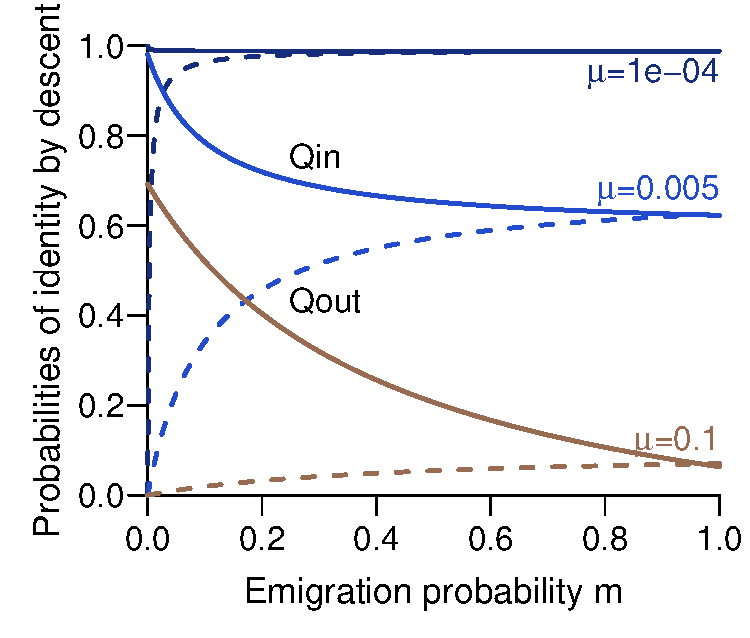
\includegraphics[width = \wpic]{../Programs/R/Pics/QplotM.pdf}}
&
\subfigure[\label{fig:sub:QWF}Wight-Fisher]{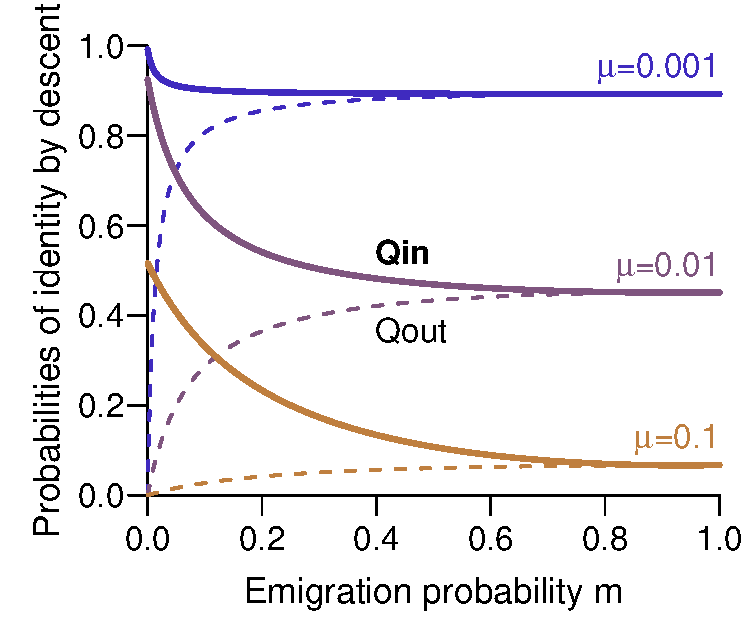
\includegraphics[width = \wpic]{../Programs/R/Pics/QplotWF.pdf}}
\end{tabular}
\caption{Probabilities of identity by descent, for two different individuals within the same deme ($\Qin$, full curves) and two individuals in different demes ($\Qout$, dashed curves), as a function of the emigration probability $m$, for different values of the mutation probability $\mu$ ($0.001$, $0.01$, $0.1$), and for the two types of life-cycles (\subref{fig:sub:QM}: Moran, \subref{fig:sub:QWF}: Wright-Fisher). Other parameters: $n=4$ individuals per deme, $\ndemes = 15$ demes. }
\label{fig:Q}
\end{figure}

Combining the formulas presented in \eqref{eq:QWF}, we obtain
\begin{equation}\label{eq:app:RWF}
R^{\WF} = \frac{(1 - \ndemes (1-m))^2 (1-\mu)^2}{\mathrm{D}^{\WF} },
\end{equation}
with
\begin{equation*}
\begin{split}
\mathrm{D}^{\WF} = & 1-\ndemes (2 (1+m (n-1))-\ndemes (1+(2-m) m (n-1)))-2 \mu \\ &+ 2 (\ndemes (\ndemes (1-m)-2) (1-m) (n-1) + n) \mu - (1-\ndemes (1-m))^2 (n-1) \mu^2.
\end{split}
\end{equation*}

When the number of demes is very large and mutation is vanishingly small, \eqref{eq:app:RWF} reduces to 
%
\begin{equation}\label{eq:app:RWFlim}
\lim_{\mu \to 0} \lim_{\ndemes \to \infty} R^{\WF} = \lim_{\ndemes \to \infty} \lim_{\mu \to 0}  R^{\WF} =  \frac{(1 - m)^2}{1 + (2 - m) m (n - 1)}.
\end{equation}
%TC:endignore 

\end{document}



